\documentclass[9pt,a4paper,fontset=windows]{ctexart}

% ===================== 页面设置 =====================
\usepackage{geometry}
\geometry{left=1.0cm,right=1.0cm,top=1.0cm,bottom=1.0cm}

% ===================== 数学公式 =====================
\usepackage{amsmath,amssymb,amsthm}
\usepackage{bm}
\usepackage{mathrsfs}
\usepackage{mathtools}

% ===================== 图表与浮动体 =====================
\usepackage{graphicx}
\usepackage{booktabs}
\usepackage{longtable}
\usepackage{float}
\usepackage{caption}
\captionsetup{font=small,labelfont=bf}

% ===================== 超链接 =====================
\usepackage[hidelinks]{hyperref}

% ===================== 其他常用宏包 =====================
\usepackage{enumitem}
\usepackage{xcolor}
\usepackage{siunitx}
\usepackage{algorithm}
\usepackage{algpseudocode}

% ===================== 定理类环境 =====================
\newtheorem{theorem}{定理}[section]
\newtheorem{lemma}[theorem]{引理}
\newtheorem{proposition}[theorem]{命题}
\newtheorem{corollary}[theorem]{推论}
\theoremstyle{definition}
\newtheorem{definition}[theorem]{定义}
\newtheorem{example}[theorem]{例}
\newtheorem{remark}[theorem]{注}

% ===================== 公式编号按节 =====================
\numberwithin{equation}{section}

% ===================== 自定义命令 =====================
\newcommand{\OR}{\mathrm{OR}}
\newcommand{\ATE}{\mathrm{ATE}}
\newcommand{\winner}{\textit{winner\_a}}
\newcommand{\tokendiff}{\textit{token\_diff\_ab}}
\newcommand{\headerD}{\textit{header\_density\_diff}}
\newcommand{\boldD}{\textit{bold\_density\_diff}}
\newcommand{\listD}{\textit{list\_density\_diff}}
\newcommand{\ability}{\textit{ability\_diff}}
\newcommand{\verbosity}{\textit{verbosity\_diff}}
\newcommand{\formatt}{\textit{format\_tendency\_diff}}
\newcommand{\longer}{\textit{longer\_a}}

% ===================== 标题信息 =====================
\title{\heiti 基于大语言模型输出文本的选择偏好研究\\
\large ——以 LMArena 人类偏好数据为例}
\author{程豪\quad 梁斯祯\quad 李嘉帅\quad 姜弼达\quad 翁祖成\quad 姚博晟\\
\small 中央民族大学理学院，北京 100081}
\date{}

\begin{document}

\maketitle
\thispagestyle{empty}

\begin{center}\small
基金项目：国家自然科学基金青年科学基金项目（72001197）；中央民族大学创新训练项目青苗计划（QMRP2025110352）\\
通信作者：程豪，E-mail：\texttt{chenghaostatistics@yeah.net}; 梁斯桢，E-mail：\texttt{largus\_liang@yeah.net}
\end{center}

% ===================== 中文摘要 =====================
\noindent\textbf{摘\quad 要：}
大语言模型的偏好对齐通常依赖人类反馈数据训练奖励模型或直接优化策略，但人类反馈中可能混入对回答长度、标题、列表、粗体等表层形式特征的偏好，使奖励模型学到“形式相似于质量”的伪相关，进而削弱对齐效果并损害模型泛化能力。现有研究多集中于“如何对齐”的方法改进，对人类反馈数据本身“在奖励什么”的系统审计仍显不足。本文以 LMArena 大规模人类偏好数据为对象，围绕长度偏差与格式偏差展开实证研究，并形成三层递进分析链：第一层通过描述统计与非参数检验识别偏好现象；第二层通过嵌套逻辑回归、调整逻辑回归、逆概率加权与倾向得分匹配，在控制任务类型、质量维度、模型能力与风格差异后估计净效应并检验稳健性；第三层通过结构方程模型分解直接路径与间接路径，讨论形式特征进入偏好判断的机制边界。研究发现：全量样本中胜者更长比例为 \(62.21\%\)，中位长度差为 \(+125\) tokens；控制混淆后，长度变量在嵌套回归 M3 中 \(\mathrm{OR}=1.3551\)，IPW 框架下 \(\mathrm{ATE}=0.1489\)。标题密度与粗体密度在控制混淆后仍保留独立正向效应，全量样本 IPW ATE 分别为 0.0277 与 0.0246；列表特征在本文采用的密度指标与控制框架下更接近长度扩张的伴生结果，不宜作为独立主结论。SEM 进一步显示，标题密度与粗体密度的直接效应 Bootstrap \(95\%\) 置信区间均排除 0，而长度直接效应区间跨 0，说明长度偏好在现象层与稳健性层最稳定，但其机制路径仍具有复合性。本文的贡献在于将偏好数据从单纯训练资源重新界定为需要审计的研究对象，建立“偏好存在性识别—净效应估计—多框架稳健性检验—路径机制解释”的连续分析链，为 RLHF 与偏好对齐中的人类反馈数据审计、奖励模型特征约束以及自动评估器校准提供可操作的实证依据。

\noindent\textbf{关键词：} 大语言模型；强化学习；偏好对齐；结构方程模型；长度偏差；格式偏差

\vspace{1em}

% ===================== 英文摘要 =====================
\begin{center}
{\heiti\large A Study on Preference for Large Language Model-Generated Text}\\[0.3em]
{\large —— Evidence from Human Preference Data in LMArena}\\[0.8em]
Cheng Hao\quad Liang Sizhen\quad Li Jiashuai\quad Jiang Bida\quad Weng Zucheng\quad Yao Bosheng\\
\small School of Science, Minzu University of China, Beijing 100081, China
\end{center}

\noindent\textbf{Abstract:}
Preference alignment of large language models (LLMs) typically relies on human feedback data to train reward models or to directly optimize model policies. However, human feedback may implicitly reward superficial formal features such as response length, headings, lists, and bold formatting, leading reward models to learn spurious correlations between surface form and underlying quality. Such biases can weaken alignment effectiveness and impair the generalization and true performance of LLMs. Existing studies have mainly focused on methodological improvements in ``how to align,'' while systematic audits of what human feedback data actually reward remain insufficient. Using the large-scale LMArena human preference dataset, this study investigates length bias and format bias through a three-stage analytical framework. First, descriptive statistics and nonparametric tests are used to identify preference phenomena. Second, nested logistic regression, adjusted logistic regression, inverse probability weighting (IPW), and propensity score matching (PSM) are employed to estimate net effects and to test robustness after controlling for task type, quality dimensions, model capability, and stylistic differences. Third, a structural equation model (SEM) is constructed to decompose direct and indirect paths and to discuss the explanatory boundary of how formal features enter preference judgments. The results show that, in the full sample, the longer response wins in \(62.21\%\) of valid pairs, with a median length advantage of \(+125\) tokens. After controlling for confounders, the length effect remains positive with M3 \(\mathrm{OR}=1.3551\) and IPW \(\mathrm{ATE}=0.1489\). Heading density and bold-text density retain independent positive effects, with full-sample IPW ATEs of 0.0277 and 0.0246, respectively. Under the density metrics and control framework used in this study, list features are better interpreted as accompanying indicators of length expansion rather than as standalone conclusions. SEM results further indicate that the Bootstrap \(95\%\) confidence intervals for the direct effects of heading density and bold density exclude zero, whereas the interval for the direct length effect crosses zero. This suggests that length preference is most stable at the phenomenon and robustness layers, but its mechanism remains composite. This study contributes by redefining preference data as an object requiring systematic audit rather than as a neutral training resource, by establishing a continuous analytical chain from preference identification to net effect estimation, multi-framework robustness checks, and path-based mechanism interpretation, and by providing empirically grounded implications for human feedback data auditing, reward model feature constraints, and automatic evaluator calibration in RLHF and preference alignment.

\noindent\textbf{Key Words:} Large Language Model; Reinforcement Learning; Preference Alignment; Structural Equation Model; Length Bias; Format Bias

\vspace{1em}

% ==================== 第一章 ====================
\section{引言}

近年来，以 ChatGPT、DeepSeek、Gemini 为代表的大语言模型已广泛用于自然语言理解、代码生成、数学推理、创意写作和人机交互等任务。随着模型从实验室环境进入真实应用场景，如何使其输出更符合人类期望，逐渐成为人工智能研究中的关键议题。无论是 RLHF 还是 DPO，其共同核心都在于把人类偏好当作高质量对齐信号，通过 RM 或偏好目标函数将“被人类选中”转化为“应该被模型学习”的行为模式。既有对齐研究通常假定人类比较选择结果能够较稳定地反映模型输出质量，但真实标注环境并不完全满足这一条件。标注者受到时间、专业知识和任务理解成本的限制，往往会借助容易识别的表面线索作出判断。回答长度、格式组织和重点标记因而可能成为“质量更高”的伪相关证据。人类偏好数据的可靠性问题由此产生。一个回答被偏好，不仅可能是因为它提供了更多准确、相关的信息，也可能是因为它长度更长、排版更整齐或“看起来”更像正式答案。两类路径在经验数据的呈现中可能高度重叠，但对 RM 的影响效果不同。本文的出发点就是尽量拆分这种重叠，考察形式特征以何种机制显著影响偏好判断。

\section{国内外研究现状}

\subsection{大语言模型偏好对齐与奖励建模研究进展}
现有对齐研究已形成 RLHF、DPO、RM 校准和自我对齐等多条技术路径。它们的共同点在于，都将人类偏好数据作为模型优化的重要依据。RM 将离散的人类选择转化为连续可比较的奖励分数，DPO 则把偏好差异嵌入策略学习目标。技术路线虽然不同，但偏好数据质量始终是影响对齐效果的关键因素。已有研究指出，RM 可能学习到与真实质量无关的捷径信号，如冗长偏差、格式偏差或谄媚性，该类问题均可以被纳入奖励破解框架：代理变量与真实目标变量之间存在偏移，优化过程会放大这种偏移。本文在这一研究脉络下，将表层形式偏好作为可操作化、可统计检验的对象，重点分析偏好数据自身是否包含可量化的表层偏差信号。

\subsection{长度偏差相关研究进展}
长度偏差是偏好对齐研究中较早受到关注的形式偏差。已有经验结果显示，人类评估者和自动评价器都可能倾向于选择更长的回答。原因在于，较长文本通常更容易给人以信息充分、回答认真或推理完整的印象，但长度增加并不必然意味着回答更准确，也不必然意味着任务完成度更高。已有研究主要从三个方面处理长度偏差：识别长度与胜率的相关关系；通过长度控制、长度匹配或后验校准降低自动评价器中的长度污染；以及构造内容相近但长度不同的对比样本，以区分冗余和质量之间的关系。与这些研究相比，本文侧重于在真实偏好数据中估计长度净效应，并进一步通过 SEM 讨论长度变量的解释边界。

\subsection{格式偏好相关研究进展}
和长度偏差相比，格式偏好更难识别。标题、列表、粗体、链接和表情符号等格式元素都可能改变回答的可读性和感知专业度。已有结果显示，部分评价器和标注者会偏好格式更丰富的回答，少量格式偏置样本也可能在偏好训练中被放大。然而，格式偏好并不能简单理解为“格式越多越好”。格式元素与回答长度、任务类型和模型风格高度耦合。例如，列表更多可能只是因为回答更长；粗体更多可能反映模型更倾向使用 Markdown；标题更多则可能对应更强的结构组织能力。因此，本文不仅考察格式计数，还构造格式密度指标，并在净效应模型中同时控制长度差和其他格式变量，以区分不同格式元素的独立贡献。

\subsection{偏好信号污染与评价偏差研究现状}
偏好信号污染并不限于长度和格式。位置偏差、确认偏误、谄媚性、认知负荷和评价器偏置都可能影响成对比较结果。对齐系统若直接使用此类数据训练，就可能继承并放大这些偏差。尤其在奖励模型或自动评价器中，表层信号往往比深层语义质量更容易学习，因而更容易成为模型优化的捷径。这类研究共同说明，偏好比较数据需要被视为待审计的研究对象，而不是天然可信的评价标准。本文的贡献在于将这一宏观判断落到具体数据和统计模型上：通过数据清洗、非参数检验、净效应估计、加权匹配和路径建模，逐层确认形式偏差的存在、强度、稳健性与机制边界。

\subsection{现有研究的不足与争议}
现有研究仍存在三方面不足。首先，一些工作更关注模型训练或偏差修正，对原始偏好数据的层级结构、字段语义和研究单位界定不够细致，统计口径容易导致偏差。其次，长度与格式偏好常被分开讨论，但真实回答中二者往往共同出现。最后，不少研究仍停留在相关性描述或单一回归估计层面，对混淆控制和机制解释的整合不够。基于上述不足，本文以 LMArena 人类偏好数据为对象，在统一框架下联合考察长度偏好与格式偏好，并按照“偏好存在性识别—净效应估计—多框架稳健性检验—路径机制解释”的递进逻辑展开分析，以补充现有研究在数据审计、混淆控制与机制分解方面的不足。

\section{研究问题与研究假设}

\subsection{核心研究问题}
本文的主要研究问题可以概括为：在 LMArena 人类偏好数据中，回答长度与格式特征是否会系统性影响人类选择偏好，并且这种影响在控制任务类型、问题维度、模型能力和模型风格后是否仍然存在。围绕这一问题，本研究还进一步关心长度、标题、列表和粗体在机制层面是否有同等地位。这一研究问题有明确的实践意义。如果偏好标签确实受形式特征影响，RLHF 和 DPO 等方法在训练时就应将长度与格式作为潜在混淆因素，予以控制和约束。结合已有研究和项目报告结果，本文提出四组假设。
\begin{itemize}[leftmargin=2em]
    \item H1：胜出回答在长度上显著长于落败回答，且长度偏好在主要任务子集中保持同向。
    \item H2：标题、列表和粗体等格式特征与偏好结果存在显著关联，但不同格式变量的稳定性不同。
    \item H3：在控制任务类型、质量维度、模型能力和风格变量后，长度偏好及部分格式偏好仍保留净效应。
    \item H4：长度差与关键格式密度差共同进入偏好形成路径，但长度变量的机制解释比标题和粗体更复杂。
\end{itemize}

\subsection{研究对象与分析思路}
本文的研究对象是 LMArena 人类偏好数据中的成对回答比较选择。研究重点是偏好与表层形式特征之间的统计关系，尤其是这种关系在多重控制后是否仍然存在。分析边界还体现在变量可得性上。本文使用的长度、格式和控制变量均来自数据集中可审计字段或分析阶段派生特征。由于缺少人工逐条内容质量评分，本研究不能完全剥离信息覆盖率、事实正确性和语义冗余等深层质量因素，因此关于长度机制的解释保持谨慎。本文按照“数据审计—变量构造—存在性识别—净效应估计—稳健性验证—路径解释”的框架展开。数据审计用来确认研究对象是否成立；变量构造用来明确形式特征如何测量；存在性识别检验偏好是否存在；净效应估计考察控制混淆后偏好是否保留；路径解释进一步讨论偏好可能通过何种机制形成。在工程流程上，项目先完成原始分片数据整合，再对各字段逐一审计。随后，将原始数据重构为优化数据，并针对任务类型完成子集划分，再分组进行描述统计与非参数检验。确认偏好显著存在后，完成净效应和稳健性分析，进一步构建 SEM 机制模型进行解释。在方法上，本文先通过分箱胜率和格式存在性统计观察现象，再采用 Wilcoxon 符号秩检验检验配对差异，并以 rank-biserial \(r\) 表示效应量。随后，使用嵌套逻辑回归考察核心效应在一步步加入控制变量后的衰减路径；使用调整逻辑回归和 IPW 从处理效应角度验证稳健性；使用 PSM 构造更平衡的处理组与对照组；最后使用 SEM 在同一模型中表达外生控制、路径层变量与偏好结果之间的路径关系。

\section{研究贡献与创新点}
在理论层面，本文将偏好数据从单纯的训练资源重新界定为需要解释和审计的研究对象。该视角强调，人类偏好并不是天然透明，其中可能同时包含内容质量判断和表层形式启发式。研究结果显示，长度、标题和粗体在偏好数据中有可量化影响，为理解 RLHF 中人类反馈的实际含义提供了经验依据。在方法层面，本文形成了一条较完整的统计实证链条。与仅进行描述性观察或单一回归不同，本研究将数据口径审计、非参数检验、效应量估计、嵌套回归、IPW、PSM 和 SEM 按研究逻辑整合起来。针对格式变量，这项研究同时使用计数和密度两个口径，以区分“格式更多”与“文本更长导致格式自然更多”。在应用层面，本文结果可以为偏好数据构建、奖励模型训练和自动评价器校准提供依据。若训练数据中的长度和结构化格式分布失衡，奖励模型可能把“更会展开”或“更会排版”误判为“质量更高”。后续数据采集可考虑长度匹配、格式平衡、样本重加权和对比样本构造，以降低表层形式特征对奖励学习的影响。

% ==================== 第二章 ====================
\section{理论分析框架与方法基础}

\subsection{偏好比较数据的功能定位与信号质量假设}
在强化学习人类反馈范式的训练流程中，偏好比较数据是连接人类判断与奖励建模的核心媒介。所谓偏好比较数据，是指由人类标注者针对同一问题的两个（或多个）候选回答，以“A 优于 B”或“B 优于 A”形式记录下来的偏序关系集合。这类数据本质上是对“相对质量”的人类判断，而非对“绝对质量”的量化评分。在 RLHF 三阶段流程中，偏好比较数据的首要用途是驱动奖励模型（Reward Model，RM）的参数学习。奖励模型通常被建模为一个序数回归或 Bradley-Terry 排名模型，接收成对回答并学习预测人类偏好概率；此后经 PPO 等策略优化算法，语言模型策略朝奖励期望最大化方向迭代更新。DPO 等方法虽然省去了显式 RM 阶段，但其核心损失函数仍然将成对偏好数据直接映射为策略参数的差异化调整，人类比较标签的质量同样是对齐效果的决定性约束。Sun 等人的自对齐工作则从另一个维度说明了这一约束的分量：在仅有不到 300 行人类标注的极度稀缺条件下，只要对齐信号足够纯粹，仍可超越多个规模更大的同期系统；反之，若信号本身受噪声污染，规模扩大反而可能加速偏差积累。

这一机制隐含着一个核心质量假设：人类偏好比较 \(\approx\) 回答质量的单调映射。即标注者选择“A 优于 B”，意味着 A 在实质意义上更符合问题的真实信息需求。若这一假设成立，奖励模型学到的就是真实质量的代理；若这一假设系统性地被违背，奖励模型学到的则可能是“外观像高质量”的表面模式，进而在对齐训练中引导语言模型向形式优化而非实质能力提升方向演化。理解偏好数据质量假设的脆弱性，需要注意两点背景约束。首先，标注者在实际评价时面临时间压力与认知负荷的双重制约，缺乏专业背景时快速可识别的表面特征（如文本更长、排版更规整）容易作为质量代理被优先采用。其次，奖励模型在训练过程中有“放大偏差”的风险：即使偏好标签只在小比例上受到形式偏差影响，经由迭代训练，模型也可能倾向于把形式特征优化强度持续推高。正是在这两个机制共同作用下，偏好比较数据中是否存在系统性形式偏差，以及这种偏差的量级与路径，成为了 RLHF 研究中不可回避的基础性问题。

\subsection{表层形式偏差的概念界定与认知成因}
“偏差”（Bias）在统计学语境中泛指估计量与真实值之间的系统性偏移。将其引入偏好数据研究语境，需要给出明确的操作性界定：所谓偏好数据中的表层形式偏差，指的是当回答在形式特征（长度、标题、列表、粗体、emoji 等）上存在差异时，这种差异性系统地影响标注结果，且这种影响并不完全通过提升回答的实质内容质量来实现。其核心特征有三：第一，该偏差是系统性的，而非随机的个人品味差异；第二，其作用路径独立于真实内容质量，即形式特征本身构成独立的偏好驱动因素；第三，它会在奖励建模与策略优化中产生下游影响，使训练出的模型优化目标偏离真实质量。需要特别指出的是，“存在形式偏差”并不等于“形式特征完全无关”。更长的回答可能确实提供了更充分的信息，更规整的格式可能确实降低了用户理解成本。本文所要区分的，是“形式改善伴随的实质质量提升”与“形式特征本身独立贡献的偏好增量”这两个不同的因果路径——正是这一区分，构成了本研究从现象识别推进到净效应估计和机制探索的核心方法论逻辑。

从认知机制角度，表层形式偏差的产生有其深刻的心理学根源。在面对复杂比较任务时，人类会自动化地启用快速认知启发（Heuristic Thinking）以降低决策成本：更长的回答更容易被直觉归类为“更完整”“更认真”；有条理的列表更容易被解读为“更有组织”“更值得信赖”；标题和粗体则通过降低认知摩擦，间接提高了内容被积极评价的可能性。这些启发式判断在日常阅读场景中往往是有效的，但在“两个回答谁更好”的强制比较任务中，当标注者无法深度校验内容准确性时，这些表面信号就可能作为质量的主要代理被系统性采用。Sharma 等人的研究将这一机制推进到了“谄媚性（Sycophancy）”层面——RLHF 训练中形式信号被奖励的效应，不只体现在格式与长度上，更会诱导模型学会迎合用户的既有信念和情感期待，使模型倾向于“看起来正确”而非“实际正确”。Wang 等人的综述则将这类多维度偏差统一纳入“奖励黑客（reward hacking）”的理论框架，指出其本质是代理奖励在高压优化下与人类真实目标之间的结构性脆弱性。这些研究共同说明，形式偏差不是偶发噪声，而是与奖励信号的设计机制深度耦合的系统性问题。

在学术分类上，偏好数据中的偏差呈现出多维结构，主要包括以下几类：长度偏差（Length Bias）——标注者对更长回答的系统性偏好；格式偏差（Format Bias）——对列表、标题、粗体等 Markdown 元素的系统性偏好；谄媚性偏差（Sycophancy）——对契合用户既有信念的回答倾向于更高评价；位置偏差（Position Bias）——对成对呈现中某一固定位置的系统性偏向；以及认知偏误（Cognitive Bias）——包括确认偏误、权威效应等个体认知层面的扭曲。这些偏差类型在真实标注场景中往往共现叠加，相互强化。本文聚焦长度偏差与格式偏差，原因在于二者与文本的可量化形式特征直接挂钩，从方法论上更易于操作化测量与系统控制。

\subsection{长度偏差的研究发展脉络与方法演进}
长度偏差是 RLHF 偏好数据研究中最早受到系统关注的问题之一。本节按研究演进的内在逻辑，梳理相关工作如何从早期的经验观察推进到方法化的识别、分解与矫正框架。在 RLHF 大规模推广之初，部分研究者已经注意到自动评价器（如 AlpacaEval 使用的 GPT-4 评价）对更长回答存在系统性偏好，但这一现象最初被视为自动评价器的具体缺陷，而非偏好数据的本质特征。Li 等人通过对人类与 32 种 LLM 偏好结构的细粒度拆解，首次将“lengthy（篇幅更长）”作为一个可量化的偏好属性独立提取，发现它在人类偏好中权重极高，而在先进 LLM 的偏好结构中权重明显偏低。这一人机偏好结构的对比，将长度偏差从“有可能存在的直觉”推进为“可统计验证的系统性现象”，确立了长度偏差研究的基本对象定义。Dubois 等人从自动评价基准设计角度提供了独立佐证，证明在控制长度后，AlpacaEval 与 LMSYS Chatbot Arena 之间的 Spearman 相关系数从 0.94 提升至 0.98，说明即使在基准层面，长度对评价结果的污染也构成了实质性干扰。

在确认现象后，研究的重点转向机制溯源——长度偏差究竟从哪里进入奖励建模链条，又如何在训练中被放大？Shen 等人的研究直接在 RLHF 训练流程内部追踪这一问题，发现奖励模型在训练过程中会习得“更长 \(=\) 更好”作为预测捷径，本质原因是训练数据中长度与偏好标签之间存在统计相关，而奖励模型无法自动区分这种相关是因果的还是虚假的；为此他们提出 Product-of-Experts（PoE）框架，将主奖励专家与长度偏差专家显式解耦。Wang 等人在反事实因果推断框架下，进一步将长度偏差归结为奖励建模中的虚假相关，指出其根本原因是代理奖励信号在高压优化下与人类真实目标的系统性偏离。Li 等人则将视角延伸至模型生成端，发现语言模型对明确长度约束指令的遵循能力本身就存在系统性不足，说明长度偏好问题同时受人类评估端启发式与模型生成端内在倾向的双重驱动。如何区分长度效应的不同来源成为了深化阶段的核心问题。Hu 等人提出将胜率分解为“可信度（desirability）”与“信息量（information mass）”两个维度的理论框架，系统阐释了长度主要通过影响信息量感知而非可信度判断来干扰评估，为区分“有效长度”与“冗余长度”提供了概念基础。在此框架下，“有效长度”增加了实质信息覆盖，理应带来偏好提升；“冗余长度”只是填充了更多词汇，其对偏好的贡献则属于形式偏差的范畴。

在识别与分解的基础上，一系列矫正方法陆续被提出，大致可分为三类。第一类是后验校准：在奖励模型训练完成后，通过估计并剥离奖励函数中的长度偏差项进行修正，代表工作是 Huang 等人的局部加权回归校准方法，在 33 个奖励模型的 RewardBench 测试中平均提升 3.11 点。第二类是训练数据去偏：在构造偏好数据时，主动通过反事实数据增强构造“内容相近、长度差异大”与“长度相近、内容差异大”两类对比对，以破坏长度与质量标签之间的虚假相关，Kim 等人的工作属于这一类型。第三类是模型级解耦：在奖励建模架构或目标函数层面显式引入长度不变性约束，Cai 等人提出的响应条件化 Bradley-Terry 模型（Rc-BT）在同一框架内同时缓解长度偏差与提升长度指令遵循能力。综合来看，长度偏差研究已经从“现象是否存在”推进到了“机制是什么”“如何矫正”的深化阶段，但对长度效应在控制任务属性与模型能力差异后的独立净效应，以及长度变量在偏好形成路径结构中所扮演角色（直接效应 vs. 间接中介 vs. 混淆代理）的系统分析，仍属研究前沿。

\subsection{格式偏差的研究演进与格式特征分类}
格式偏差的研究发展与长度偏差有相似的演进逻辑，但面临更为复杂的测量挑战：格式特征本身与长度、任务类型和模型风格高度耦合，若不加以区分，格式偏差研究很容易退化为长度偏差研究的另一种表述形式。所谓“响应格式”，在大语言模型输出语境下通常指 Markdown 语法元素，包括多级标题、有序与无序列表、粗体、斜体、代码块以及 emoji 等视觉元素。这些元素的共同特征是在不直接改变文本信息内容的情况下，影响文本的视觉呈现与可读性组织。Do 等人的系统研究从操作层面对格式类型进行了规模化梳理，测试了多选、列表、映射等 15 种常用格式，在 8 类生成任务上均发现了显著的格式敏感性，ChatGPT 在不同格式间的性能方差最高达 235.33，经格式微调后可降至 0.71 以下。这说明格式不只是偏好偏差的来源，也是影响模型实际能力表现的系统性变量。

格式偏差的核心来源在于，格式化元素可以通过降低认知摩擦（如标题快速定向）和提升可信感（如分点作为“理性整理”的信号）来影响评价者判断，而不论其背后的内容质量如何。Zhang 等人的研究是这一领域的奠基性工作之一，他们通过数据注入实验证明，在去偏的偏好数据集中混入不足 1\% 的格式偏置样本，即可通过迭代 DPO 和 PPO 训练在模型行为层面放大为显著的格式偏差。这也说明偏好数据中的格式污染对下游训练有高度非线性放大效应，不能以“污染比例低”为由轻视。Park 等人则进一步揭示，当低质量回答采用更具修辞吸引力的格式时，评判模型的判断准确率会显著下降；在风格相似条件下则相对准确——表明格式偏差的触发有条件性，在不同回答格式差异悬殊时才会系统性干扰判断，这为识别格式效应的边界提供了重要参照。

格式偏差研究的核心方法论挑战，在于格式特征计数与文本长度之间的内在耦合。一篇更长的回答自然有更多空间容纳标题、列表和粗体标记，如果直接以绝对计数作为格式变量，那么“更多格式”几乎等价于“更长文本”，格式效应就会被长度效应完全混淆。为此，研究者普遍转向格式密度（Format Density）指标，即单位 token 数内的格式元素出现频率，将格式的“浓度”与“总量”加以区分。这一操作化转变是格式偏差从描述性研究推进到控制混淆后的稳健性分析的关键方法论步骤，也揭示了一个重要的研究预期：不同类型格式元素在密度分析下可能表现出截然不同的结论，部分格式的“优势”可能仅是长度扩张的伴生现象，而非独立偏好信号。从 NLP 模型对虚假相关性依赖的认知机制看，格式特征与偏好标签的耦合正是这类虚假相关性的典型体现。

Gan 等人提出的 BiAxisAudit 框架揭示了格式偏差更深层的复杂性：偏差不仅存在于对两个回答的选择层面（即哪个被选中），也存在于对单一回答的展开层面（即如何组织语言来描述内容）；这两个层面的偏差方向甚至常常不一致，仅在选择层面测量的 RLHF 偏好数据可能系统性地遗漏只在展开层浮现的格式效应。Koo 等人则从 LLM-as-a-Judge 角度系统测量了模型评价器的认知偏误，发现平均 40\% 的比较判断存在偏误，人机偏好秩相关度均值仅为 44\%，说明格式偏差的感染范围不局限于人类标注，也延伸至模型评价链条。Ye 等人将格式冗余、谄媚性与顺从语气统一视为偏好奖励学习中的“捷径行为（shortcut behaviors）”，提出 PRISM 方法通过群不变核学习加以矫正，为格式偏差的概念化提供了新的理论坐标——它不只是一个评测层面的技术问题，而是模型在偏好学习中对表层捷径的系统性依赖。

\subsection{混淆控制与识别框架}
长度偏差与格式偏差的研究面临一个共同的方法论障碍：原始相关性无法直接用来净效应推断。在真实偏好数据中，长度、格式与偏好结果之间的原始相关，往往被模型能力差异、任务类型分布和风格倾向等混淆变量所放大或扭曲。这样一来，识别形式特征的独立净效应，需要系统性的混淆控制策略与多框架验证逻辑。

在本文的研究语境中，混淆路径主要来源于三个维度。其一，模型能力差异（ability\_diff）：能力更强的模型往往同时在内容质量和输出风格上占优，这使得“能力 \(\rightarrow\) 回答更长或格式更好 \(\rightarrow\) 更受偏好”构成了一条额外传导路径，混淆了长度与格式的独立效应。其二，冗长风格（verbosity\_diff）：不同模型有内在不同的输出长度倾向，这种训练先验会系统性影响长度差的分布，如不加控制，长度净效应估计就会偏高。其三，任务类型（category tags）：代码、数学、创意写作等不同任务对回答长度的客观需求存在显著差异，如果任务类型分布不均衡，粗长度效应就会受到任务结构的额外影响。

逻辑回归（logistic regression）是控制混淆、识别净效应的基础工具。在本文中，嵌套逻辑回归的核心设计思路是“分层推进而非一次性控制”：先建立仅含核心解释变量的粗模型（M0/F0），再分层加入任务类型（M1/F1）、质量维度（M2/F2）、模型能力与风格代理变量（M3/F3），观察核心系数（OR）在层层控制中如何变化。这一设计的意义不只在于给出最终净效应数字，更在于记录混淆去除的过程——某个偏好效应被控制变量解释掉多少，直接提供了“原始相关中有多少是虚假的混淆贡献”的测量依据。

倾向得分（Propensity Score）方法是观测研究中模拟随机化的核心手段之一。逆概率加权（Inverse Probability Weighting，IPW）通过为每个观测单元分配与其倾向得分成反比的权重，构造一个对观测协变量分布更均衡的“伪总体”，从而在无法进行实验随机分配的条件下，获得更接近准因果视角的平均处理效应估计（Average Treatment Effect，ATE）。稳定化权重（stabilized weights）可防止少数极端倾向得分个体主导结果；有效样本量（ESS）则作为权重分布是否合理的诊断指标。

与 IPW 不同，倾向得分匹配（Propensity Score Matching，PSM）通过为每个处理组样本找到倾向得分相近的对照组样本，直接构造可比样本对，再在这些更可比的样本上估计处理效应。1:1 最近邻匹配结合 caliper 约束（即限制最大匹配距离），既保留样本规模，也提高每对匹配的可比性。标准化均值差（Standardized Mean Difference，SMD）是判断匹配质量的核心指标——它衡量处理组与对照组在每个控制变量上的分布差异，不依赖样本量，能直接反映协变量均衡程度。本文把“匹配前后 mean\(|\)SMD\(|\) 显著下降”与“匹配后效应仍成立”视为联合稳健性证据。

上述方法主要解决“偏好效应是否真实存在”的问题，而结构方程模型（Structural Equation Modeling，SEM）的引入，是为了进一步回答“这些效应如何进入偏好判断”。SEM 允许同时建模多条直接效应路径与通过路径层变量的间接传导关系，并在统一框架下分解总效应的来源。本文使用的是观测变量路径模型，而非潜变量测量模型，即所有变量均为可直接测量的观测量，不假设存在隐含因子。路径方向的设定基于前序分析的理论预期：能力差与风格差作为外生变量影响长度与格式特征，长度差与格式密度差作为路径层变量影响最终偏好。Bootstrap 区间用来对间接效应乘积的非对称分布进行鲁棒推断。需要特别指出的是，SEM 路径解释的边界是“理论一致、统计上可支持的传导结构”，而非严格实验意义上的因果定论。

本文将嵌套逻辑回归、IPW、PSM 和 SEM 置于同一分析链而非孤立使用，背后是一种“多框架交叉验证”的稳健性逻辑：若某一偏好效应在多种方法论假设下（参数回归 vs. 重加权 vs. 匹配 vs. 路径分析）均保持一致，则可认为该效应对单一方法的设定假设不敏感，有更强的结论可信度。反之，若某效应仅在特定方法框架下显现，则需要对其可靠性保持审慎。

\subsection{理论分析框架与研究假设}
综合前述文献脉络与方法论讨论，本文将偏好形成过程概括为“任务与模型差异—表层形式特征—偏好结果”的三层结构。外生层包括任务类型、质量维度、模型能力差与风格差；路径层包括长度差、标题密度差、粗体密度差，并将列表密度保留为敏感性变量；结果层为 \winner。该框架既承认任务需求与模型差异会影响回答形式，也检验形式特征在控制前者之后是否仍保留独立贡献。在这一框架下，H1 对应长度偏好的存在性，H2 对应格式效应内部的分化，H3 对应控制混淆后的净效应保留，H4 对应路径层面的机制解释。本文后续章节将按“先确认现象，再识别净效应，再讨论路径”的顺序依次展开。

% ==================== 第三章 ====================
\section{数据来源与预处理}

\subsection{数据来源与原始结构}
本文使用的数据来自 LMArena 人类偏好数据，呈现为成对比较记录。原始数据以 7 个 parquet 分片形式存储，文件名为 train-00000-of-00007 至 train-00006-of-00007。将 7 个分片统一整合后，共得到 135,634 条记录、14 个顶层字段，覆盖 53 个参与比较的模型。项目早期就对分片完整性进行审计，结果发现同一 evaluation\_session\_id 会跨文件重复出现，这也说明原始分片只是存储切分，而不是会话边界上的自然切分。这样一来，若不先整合成统一总表，就无法正确识别同一会话内部的评价次序与上下文关系。

从字段构成看，原始数据的 14 个顶层字段分别为 id、model\_a、model\_b、winner、evaluation\_session\_id、evaluation\_order、conversation\_a、conversation\_b、full\_conversation、conv\_metadata、category\_tag、language、is\_code 和 timestamp。它们大体可以分为四类：第一类是比较识别字段，包括样本 id、模型 A/B 名称以及 winner，用来指明一条偏好比较记录的基本对象和胜负结果；第二类是会话定位字段，包括 evaluation\_session\_id 与 evaluation\_order，用来表征该条比较位于哪一个用户会话及该会话中的第几轮评价；第三类是对话主体字段，即 conversation\_a、conversation\_b 与 full\_conversation，用来保存用户与两个候选回答之间的实际对话内容；第四类是辅助元数据字段，包括 conv\_metadata、category\_tag、language、is\_code 与 timestamp，用来提供 token 汇总、任务标签、语言标记、代码任务标记和时间信息。这种结构说明，原始数据并不是一个只包含“提示词 \(+\) 两个回答 \(+\) 胜者”的极简成对样本表，而是把比较行为嵌入在更完整的交互上下文中。

进一步看对话结构，conversation\_a 与 conversation\_b 均不是单个字符串，而是列表形式的消息序列。审计结果显示，两侧 role 都只有 user 与 assistant 两种取值，且各自都累计出现 171,054 次，合计形成 342,108 个 segment。每个 segment 内部又包含 content 子结构；从实际分布看，绝大多数 content 长度均为 1，次级字段几乎统一表现为 type="text" 与 text，这也说明原始数据本质上是文本对话记录，而非图文混合或多模态数据。conversation\_a 中仅有 109 个 segment 的 content 为空，conversation\_b 中为空的 segment 为 91 个，总体占比很低，但这些异常值若不清理，仍会影响后续文本长度和格式统计的稳定性。更重要的是，conversation\_a 与 conversation\_b 各自保留了同一轮比较下的完整对话链，这也说明模型 A 与模型 B 并不是只提供一个独立回答，而是在共享用户输入轨迹的基础上，分别形成了各自的回答路径。

从层级关系上看，原始数据呈现出明显的 Session、Order、Turn 三级嵌套结构。evaluation\_session\_id 的唯一值总数为 115,372，其中有 13,206 个 session 出现了不止一次，涉及 33,468 行记录，占总样本的 24.68\%，说明相当一部分用户会话包含多轮评价。进一步看 evaluation\_order，该字段共有 28 个不同取值，其中 order=1 的记录为 108,315 行，order=2 为 15,972 行，之后随轮次升高快速递减，最高达到 28。也就是说，一行数据并不等于“一个独立问题的一次性比较”，而更接近于“某个会话中某一轮 order 上的一次双回答偏好判断”；在每个 order 内部，conversation\_a 与 conversation\_b 又继续按 turn 展开为 user/assistant 交替消息。正因为原始研究对象有这种分层嵌套特征，后续分析如果直接把整表视为平铺样本，就会把会话级历史、order 级比较与 turn 级文本混杂在一起，导致变量口径失真。

除对话字段外，conv\_metadata 与 category\_tag 是原始数据最关键的两个结构化辅助字段。conv\_metadata 在 135,634 行中无一缺失，至少稳定包含 sum\_assistant\_a\_tokens、sum\_assistant\_b\_tokens、sum\_user\_tokens、context\_a\_tokens 与 context\_b\_tokens 五类 token 汇总信息，为后续长度变量构造提供了原始来源。category\_tag 同样在整表中保持稳定字典结构，内部包含 creative\_writing\_v0.1、if\_v0.1、math\_v0.1 以及 criteria\_v0.1 等子模块，可同时提供任务标签与七个质量维度标签；同时，顶层 language 字段共有 126 种取值，is\_code=True 的记录有 39,363 行，说明该数据集在语言和任务类型上都有较强异质性。总体而言，原始数据并不是一个已经“天然适合回归分析”的整洁表，而是一个保留了真实平台交互痕迹的层级化比较数据对象。第三章后续所有清洗、重组与变量派生工作，正是为了把这一复杂结构转换为口径一致、可统计建模的研究样本。

\begin{figure}[htbp]
\centering
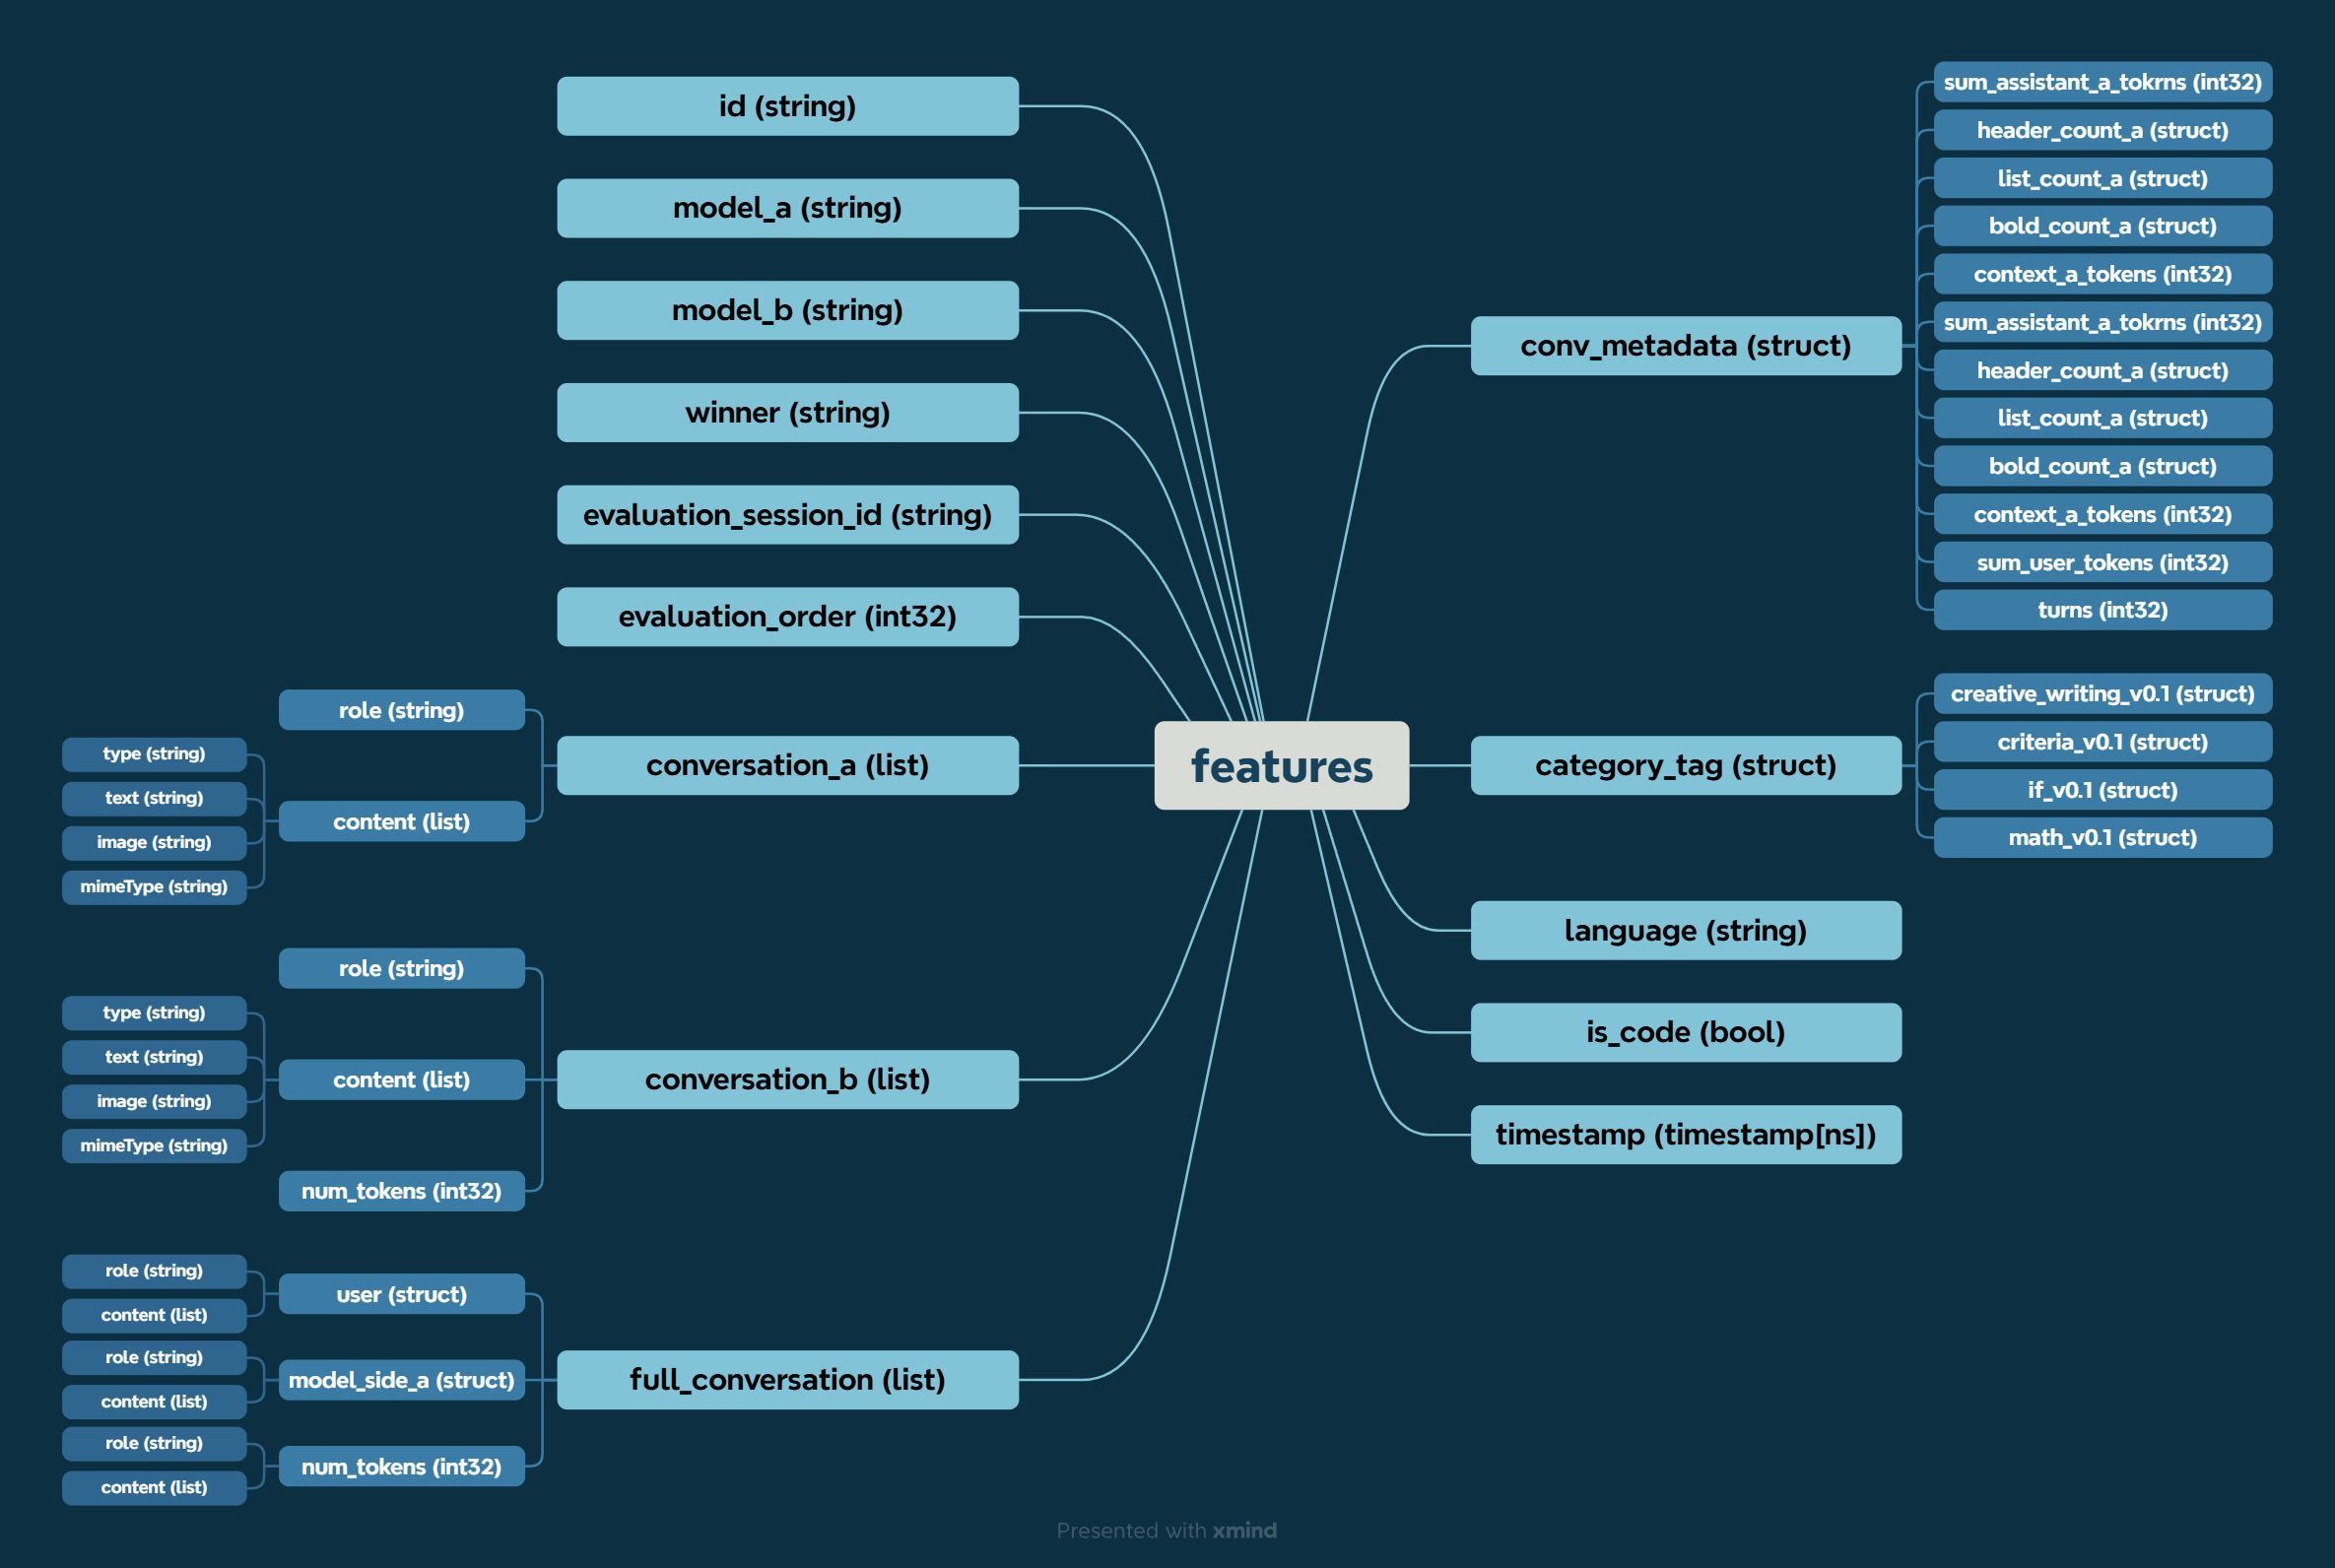
\includegraphics[width=0.9\textwidth]{figures/P01_original_structure.png}
\caption{原始数据结构图}
\label{fig:original_structure}
\end{figure}

\subsection{数据审计与清洗规则}
在字段摸底阶段，本文重点检查了评价轮次与 token 汇总字段之间的对应关系。审计结果显示，conv\_metadata 中的 sum\_user\_tokens 在首轮评价时能够准确对应当前轮次 user 消息的 token 总和，但在高阶 order 中开始累计此前会话历史，从而不再表示当前比较单元的真实输入长度。由于长度变量是本研究的核心解释变量之一，这种口径漂移会直接破坏测量一致性。这样一来，仅保留 evaluation\_order \(=1\) 并不是经验性删样，而是基于测量效度作出的方法学决策。首先，一致性审计表明，order \(=1\) 的 108,315 条记录中，sum\_user\_tokens 与当前轮次 user 消息 token 总和完全一致；而 order \(>1\) 的 27,319 条记录全部发生失配，说明高阶轮次的汇总字段已经掺入会话历史。其次，污染有明确的量级扩张特征。sum\_user\_tokens 的均值从 order \(=1\) 的 138.68 tokens 上升到 order \(=2\) 的 210.18 和 order \(=3\) 的 300.31；但对应当前轮次 user token 的均值仅为 138.68、84.29 和 90.88，意味着高阶 order 的汇总字段相对当前轮次分别膨胀至 2.49 倍和 3.30 倍。全样本中，evaluation\_order 与 sum\_user\_tokens 的 Pearson 相关为 0.1391（\(p<0.001\)）。这种污染并不是零星异常，而是与轮次口径系统绑定：order \(>1\) 记录的失配率为 \(100\%\)，order \(=1\) 记录的失配率为 \(0\%\)。

\subsection{优化主表构建与样本筛选}
在上述审计基础上，本文在整合后的 135,634 条记录中最终保留 108,171 条，过滤 27,463 条，保留率为 \(79.75\%\)。其中，evaluation\_order \(>1\) 的污染样本为 27,319 条，是最主要的过滤来源；其余过滤原因包括空内容、语言异常和关键标签缺失。清洗后的主表采用 nested schema，而非早期扁平化的宽表组织方式。具体而言，对话文本被整理为 conv\_a、conv\_b、conv\_user，token 与格式统计被整理为 metadata\_a、metadata\_b、metadata\_user，任务标签和质量维度则分别整理为 category\_tag 与 criteria。

\begin{figure}[htbp]
\centering
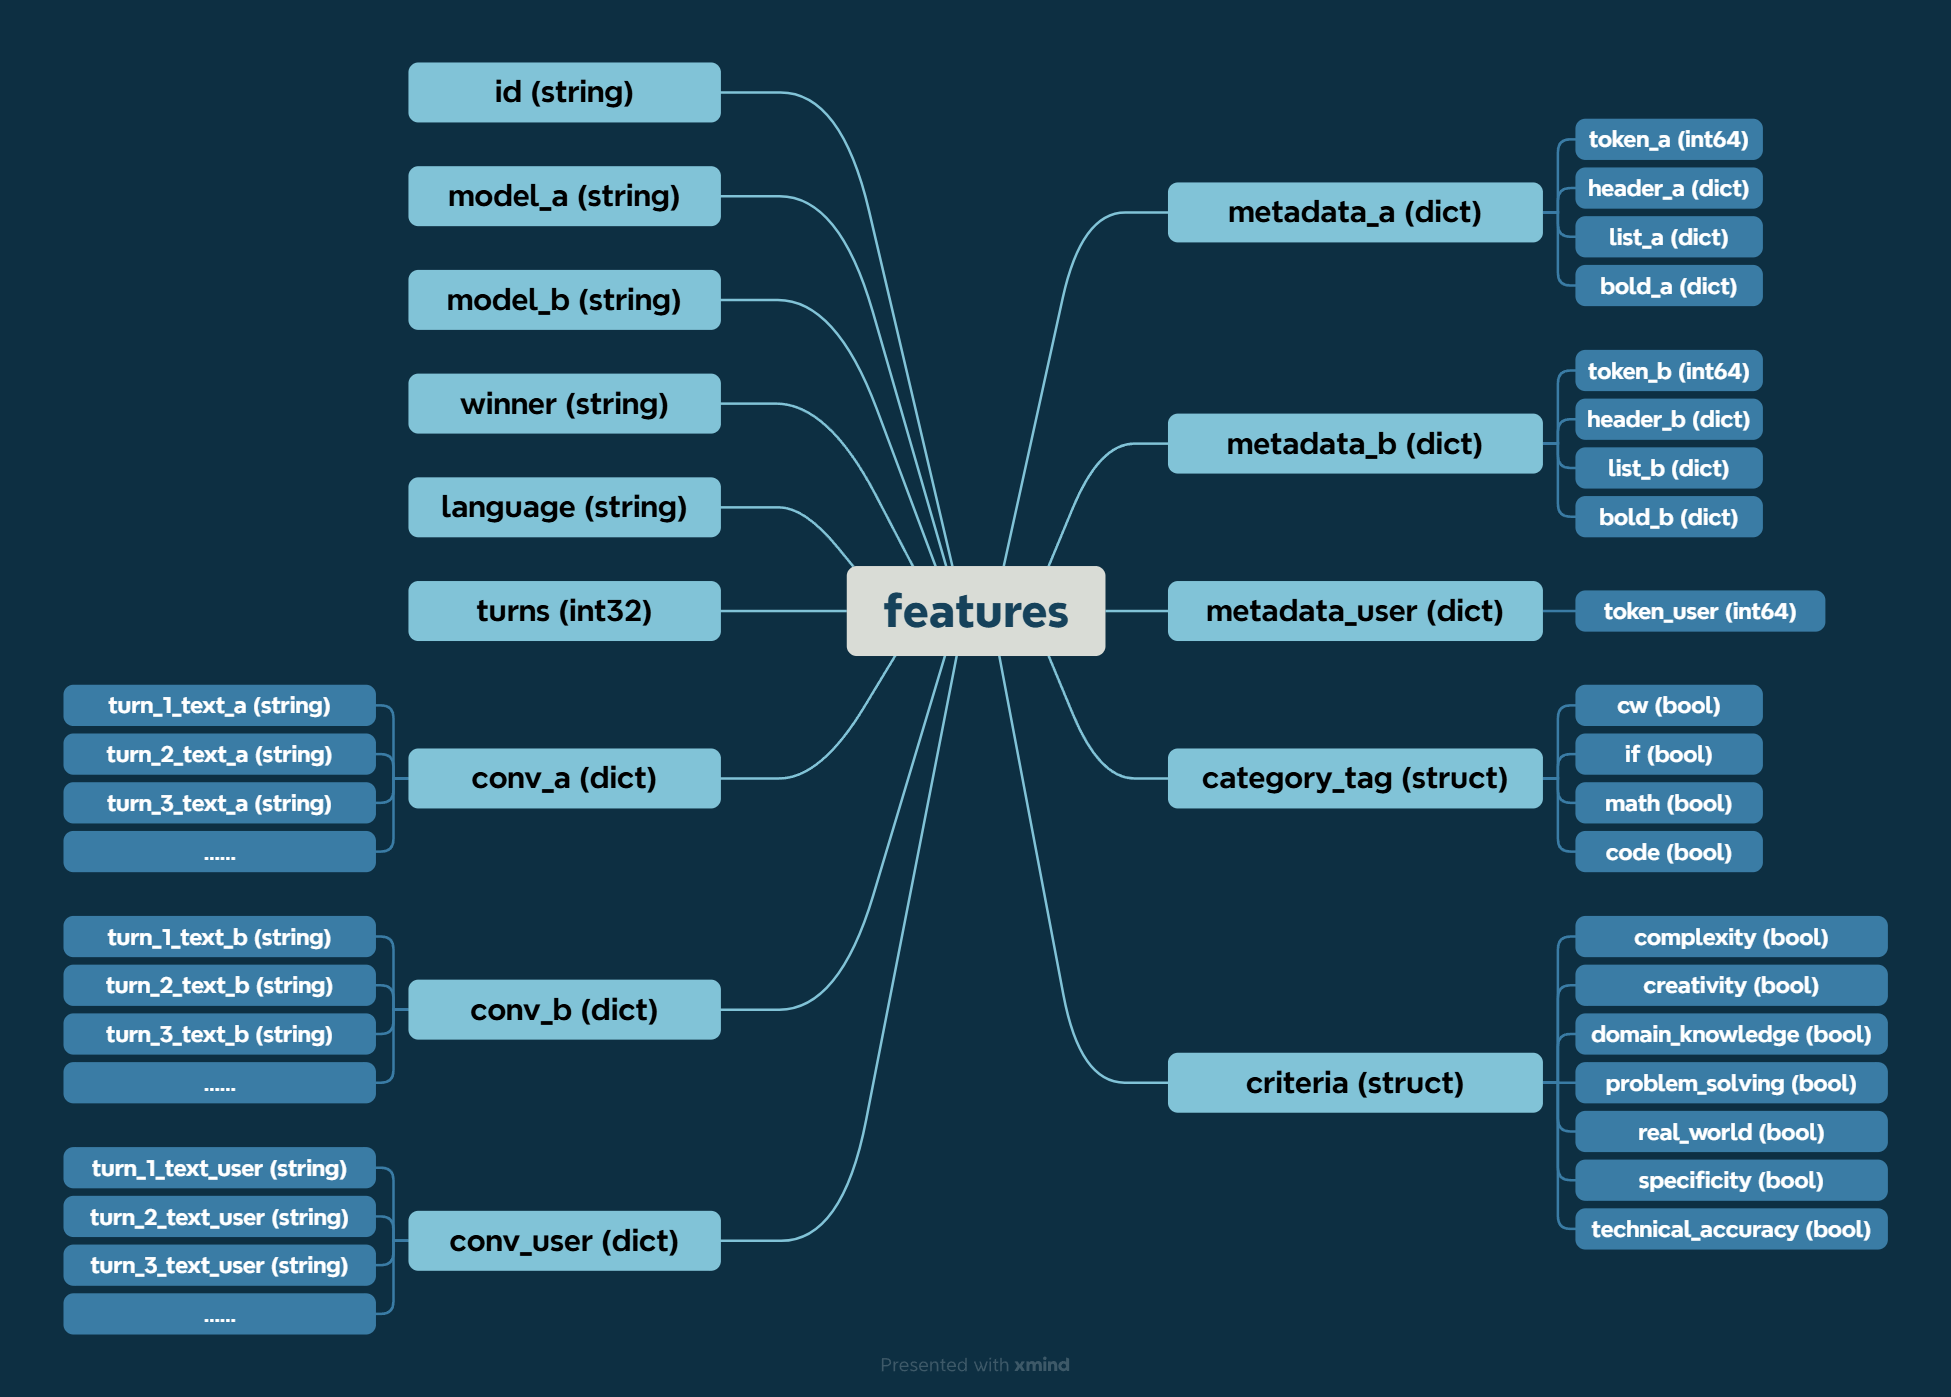
\includegraphics[width=0.9\textwidth]{figures/P03_optimized_structure.png}
\caption{优化数据结构图}
\label{fig:optimized_structure}
\end{figure}

\begin{table}[htbp]
\centering
\caption{样本筛选流程汇总}
\label{tab:sample_filter}
\begin{tabular}{lll}
\toprule
阶段 & 样本量 & 说明 \\
\midrule
原始整合记录 & 135,634 & 七个 parquet 分片合并后的总样本 \\
保留 evaluation\_order \(=1\) & 108,315 & 剔除高阶轮次造成的长度口径污染 \\
清洗后优化主表 & 108,171 & 进一步剔除空内容、语言异常和关键标签缺失 \\
偏好方向分析样本 & 78,970 & 排除 tie 与 both\_bad 后的有效配对 \\
\bottomrule
\end{tabular}
\end{table}

注：表 \ref{tab:sample_filter} 中的样本筛选顺序依次为轮次过滤、内容清洗与胜负标签过滤。最关键的口径判断是：27,319 条 evaluation\_order \(>1\) 记录全部存在 sum\_user\_tokens 与当前轮次 user token 总和不一致的问题，因而不宜继续作为长度分析样本使用。

这种结构调整有两个好处。首先，主表只保留稳定的顶层字段，把长度差、格式密度差等分析变量留到下游按需派生，避免主表被脚本级临时变量不断污染。其次，nested schema 使会话对象、回答对象和标签对象之间的边界更清晰，便于后续脚本共享同一套访问口径。

\subsection{任务子集划分}
在优化主表基础上，本文还进一步划分出 20 个任务子集，包括 4 个可重叠的单类子集和 16 个互斥纯净分区。四类布尔任务标签分别为 creative\_writing、if、math、code。这样的设计允许本研究同时从两个层面观察偏好差异：一方面，通过单类子集观察某一任务属性出现时的总体模式；另一方面，通过纯净分区更严格地比较不同任务组合下的异质性表现。

% ==================== 第四章 ====================
\section{变量构造与研究设计}

\subsection{结果变量与长度相关变量}
本文的核心结果变量为 \winner，即在每一对比较中 A 侧回答是否获胜。长度相关变量包括 a\_tokens、b\_tokens 及其差值 \tokendiff。在部分稳健性分析中，还进一步构造了二元处理变量 \longer，表示 A 是否比 B 更长。这样设计后长度既可以作为连续差值进入净效应模型，也可以作为处理变量进入调整逻辑回归、IPW 和匹配分析。

\subsection{格式变量与密度指标构造}
格式变量主要包括标题、列表和粗体三类计数特征，分别记录两侧回答中的出现情况及差值。考虑到格式绝对计数与文本长度高度耦合，本文还进一步构造格式密度变量。实现上，密度定义为 \(\text{count\_f} / \max(\text{tokens},1)\)，在代码中通过 clip(lower=1) 实现，用来防止极端情况下出现零分母。需要指出的是，在 108,171 条优化样本中，A、B 两侧均未出现 0 token 回答，因而该处理属于防御式实现，不会实质改变结论。采用密度而非绝对计数的目的，是将“格式更多”与“因为更长所以自然更容易出现格式”区分开来，从而使格式偏好分析不至于退化为长度偏好的重复表达。

\subsection{任务类型、质量维度与模型代理变量}
为控制问题层面的差异，本文使用了 creative\_writing\_bool、if\_bool、math\_bool、code\_bool 四个任务类型变量，以及从 category\_tag 中抽取出的 7 个质量维度，如 complexity、creativity、domain\_knowledge、problem\_solving、real\_world、specificity、technical\_accuracy 等。为控制模型层混淆，本研究构造了 \ability、\verbosity、\formatt 三个代理变量，其实际口径分别为 win\_rate\_a \(-\) win\_rate\_b、mean\_tokens\_a \(-\) mean\_tokens\_b 和 mean\_format\_a \(-\) mean\_format\_b；其中 win\_rate、mean\_tokens 和 mean\_format 均由全量 optimized\_data 计算的模型历史统计量映射而来，mean\_format 表示标题、列表与粗体总格式元素数的平均值。这些变量的重要性在于，模型能力、风格和任务属性本身都可能同时影响“回答更长”与“回答更容易获胜”，若不把它们纳入控制项，长度和格式的粗效应就可能被系统性高估。本文为避免子集样本量过小导致代理量剧烈波动，采用全量样本一次性估计后再映射到配对层，不在各子集内重估。与此同时，本研究并未对这些模型统计量采用留一法或交叉验证，因而它们应被理解为全局描述性代理变量，而非外部验证的预测特征。

\begin{table}[htbp]
\centering
\caption{核心变量定义}
\label{tab:variables}
\begin{tabular}{lll}
\toprule
变量名 & 定义 & 角色 \\
\midrule
\winner & A 侧是否在配对中获胜 & 结果变量 \\
\tokendiff & A、B 回答 token 数之差 & 长度净效应 / SEM \\
\longer & A 侧是否比 B 侧更长 & 处理变量（IPW / PSM） \\
\headerD & 标题密度差 & 格式主分析 / SEM \\
\boldD & 粗体密度差 & 格式主分析 / SEM \\
\listD & 列表密度差 & 敏感性分析 \\
\ability & 模型整体胜率差 & 模型层控制 \\
\verbosity & 模型平均长度倾向差 & 模型层控制 \\
\formatt & 模型平均格式倾向差 & 模型层控制 \\
criteria & 七维 complexity 等 7 个质量维度 & 题目层控制 \\
\bottomrule
\end{tabular}
\end{table}

注：表 \ref{tab:variables} 中三个模型层代理变量均由全量 optimized\_data 一次性估计后映射到配对层，不在子集内重估；它们用于控制模型能力与风格差异，而不是构造独立的外部评分。

\subsection{分析方法链设计}
本文整体采用四层递进方法链。第一层是描述统计与趋势分析，用来确认偏好现象是否存在。第二层是 Wilcoxon 检验、Bootstrap 区间和效应量分析，用来把可视化趋势推进为正式统计结论。第三层是嵌套逻辑回归、调整逻辑回归、逆概率加权和倾向得分匹配，用来控制混淆并检验稳健性。第四层是结构方程模型，用来讨论变量之间的直接路径和间接路径。这一设计的基本逻辑在于：先证明现象真实存在，再证明它不只是显著性假象，接着证明它不依赖单一估计框架，再尝试解释偏好形成机制。

\subsection{核心统计方法的适用性说明}
为了避免方法部分只剩下“报结果”，本节进一步说明各统计工具在本文中的识别任务。描述统计与趋势分箱主要回答“现象是否肉眼也能看出”，如长度差值分箱后的胜率曲线，能够先确认偏好是否有稳定方向。Wilcoxon 符号秩检验则回答“配对差值的中位数是否系统性大于 0”。由于本研究的核心数据天然是成对比较，且 token 差、格式计数差和密度差都存在明显偏态和长尾特征，因而使用基于秩的非参数检验比配对 \(t\) 检验更稳健，也更符合本数据的分布形态。

Bootstrap 区间在本文中的作用，不是替代主检验，而是补充“差值大概落在什么范围内”。显著性只说明是否偏离 0，不能说明偏差的量级与不确定性，因而本研究对中位长度差、处理效应和路径效应都配套报告 Bootstrap \(95\%\) 置信区间。效应量方面，Wilcoxon 主检验主要配套 rank-biserial \(r\)，用来描述秩差异的强弱；Cohen's \(d\) 和 Hedges' \(g\) 仅作为参数化近似参考，不承担主结论功能。

逻辑回归部分的任务是把“偏好现象存在”推进为“控制混淆后是否仍存在”。由于 \winner 是二值结果变量，线性回归既不适合概率边界，也不便于解释胜出概率与多组控制变量之间的非线性关系，因而本文采用了 logit 链接函数建模。嵌套逻辑回归中的 M0 到 M3、F0 到 F3 并不是重复估计，而是通过分层加入控制变量，观察核心系数从粗效应到净效应如何衰减。这里的 OR 反映赔率比，OR 大于 1 表示相应变量增加会提高 A 侧获胜赔率；AME 反映平均概率变化，便于把赔率语言翻译成更直观的概率语言；Wald 则用来给出局部效应强度的标准化近似。

IPW 和 PSM 负责回答“如果把处理组和对照组在观测协变量上尽量变得可比，结论是否仍成立”。IPW 通过倾向得分为样本重新赋权，构造一个更接近随机分配的伪总体，并以 ATE 作为平均处理效应指标。本文使用了稳定化权重，并配套报告 ESS，以检查是否存在少数极端权重主导结果。PSM 则用 1:1 最近邻匹配直接构造可比样本对，再通过 SMD 诊断匹配前后平衡性是否改善。本研究把 mean(SMD) 是否显著下降，以及匹配后配对 Wilcoxon 是否仍显著，作为匹配诊断是否成立的联合标准。

SEM 的角色与前述方法不同。它不是再做一轮“显著性复核”，而是把能力差、风格差、长度差和格式密度差放进同一个路径框架中，考察它们是直接作用于偏好，还是先通过中介层传递到偏好。本文采用的是观测变量路径模型，而非潜变量测量模型，因而关注重点不在量表信度，而在路径结构是否合理、路径方向是否与前序分析一致，以及直接效应、间接效应和总效应如何共同构成偏好形成机制。

% ==================== 第五章 ====================
\section{偏好存在性分析与检验}

\subsection{长度偏好的描述性特征}
长度偏好的最直观现象是，胜出回答往往更长。全量样本的 Wilcoxon 检验基于 78,970 个有效配对，其中胜者更长的对数为 49,129，对应比例为 \(62.21\%\)；中位长度差为 \(+125\) tokens，Bootstrap \(95\%\) 置信区间为 \(+121\) 至 \(+130\) tokens。无类别样本和代码样本中，这一趋势同样明显，其中仅代码子集的中位长度差达到 \(+203\) tokens，指令加代码子集甚至达到 \(+256\) tokens。对照来看，仅数字子集（\(+56\) tokens）和仅创意写作子集（\(+60\) tokens）的中位长度差相对较小，反映出不同任务类型对回答长度的需求差异显著。无类别子集的胜者更长比例为 \(63.72\%\)，中位长度差为 \(+121\) tokens，与全量走势基本吻合。

从这些结果能看出，长度偏好不是少数极端样本带来的局部现象，而是在多个任务配置下都重复出现的总体模式。这至少说明，更长的表达在比较场景中确实有稳定优势，但此时还不能直接解释为“长度本身就是质量”。

\begin{figure}[htbp]
\centering
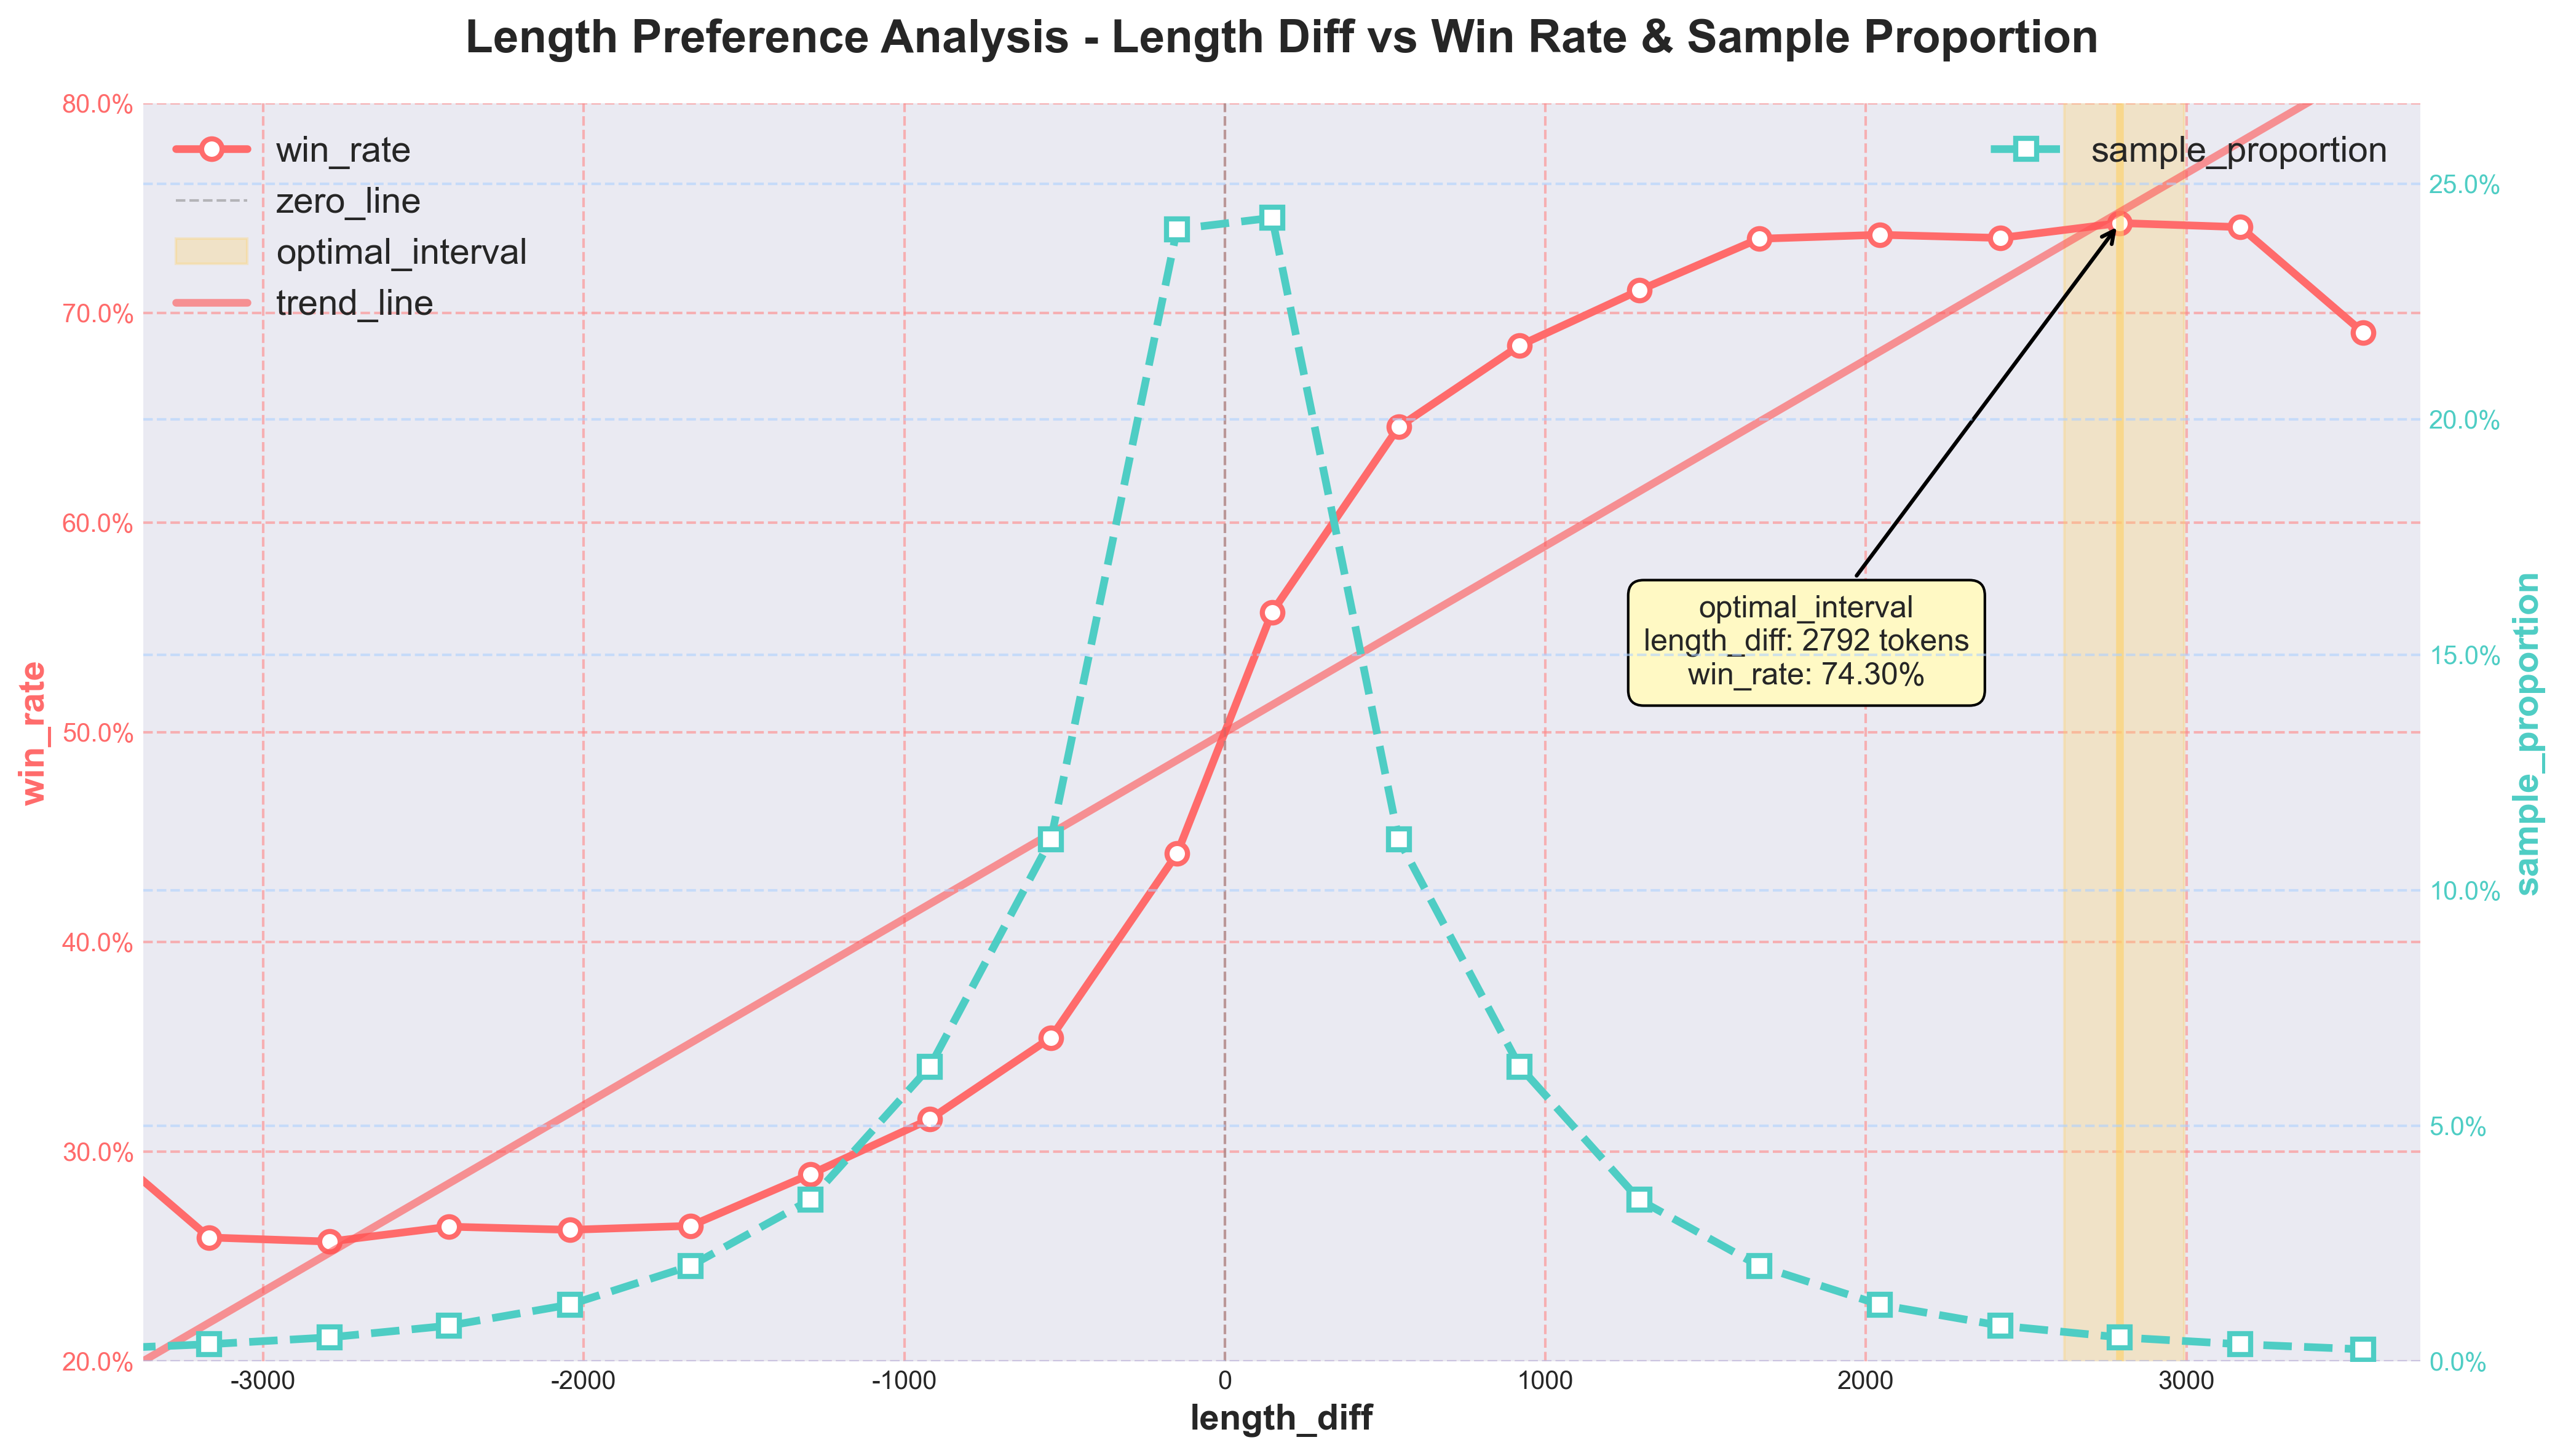
\includegraphics[width=0.9\textwidth]{figures/P04_01_full_length_diff_line_chart.png}
\caption{全量样本长度差与胜率、样本比例趋势图}
\label{fig:length_pref}
\end{figure}

注：图 \ref{fig:length_pref} 横轴为 A 侧与 B 侧的 token 数差异，纵轴为 A 侧获胜概率。该图用于展示长度差扩大时胜率如何变化，主要承担趋势识别功能，而非因果解释。

\subsection{格式偏好的描述性特征}
格式偏好的描述性结果显示，胜者在标题、列表和粗体计数上都更可能占优。以全量样本为例，胜者标题更多的比例为 \(35.02\%\)，列表更多的比例为 \(50.14\%\)，粗体更多的比例为 \(52.16\%\)。单看计数差，这三类格式变量都与胜率存在正向关联。但把分析从绝对计数推进到密度层面后，不同格式变量开始分化。全量样本中，标题密度差的辅助 Wilcoxon 检验 \(p\) 值为 \(6.9\times 10^{-111}\)，粗体密度差的 \(p\) 值为 \(2.1579\times 10^{-277}\)，均显示出稳定差异；而列表密度差的 \(p\) 值为 0.11961，不再显著。这也说明“胜者更常使用列表”这一现象，很可能更多来自回答更长、更展开时自然携带的列表，而不是列表本身带来的独立优势。

\begin{figure}[htbp]
\centering
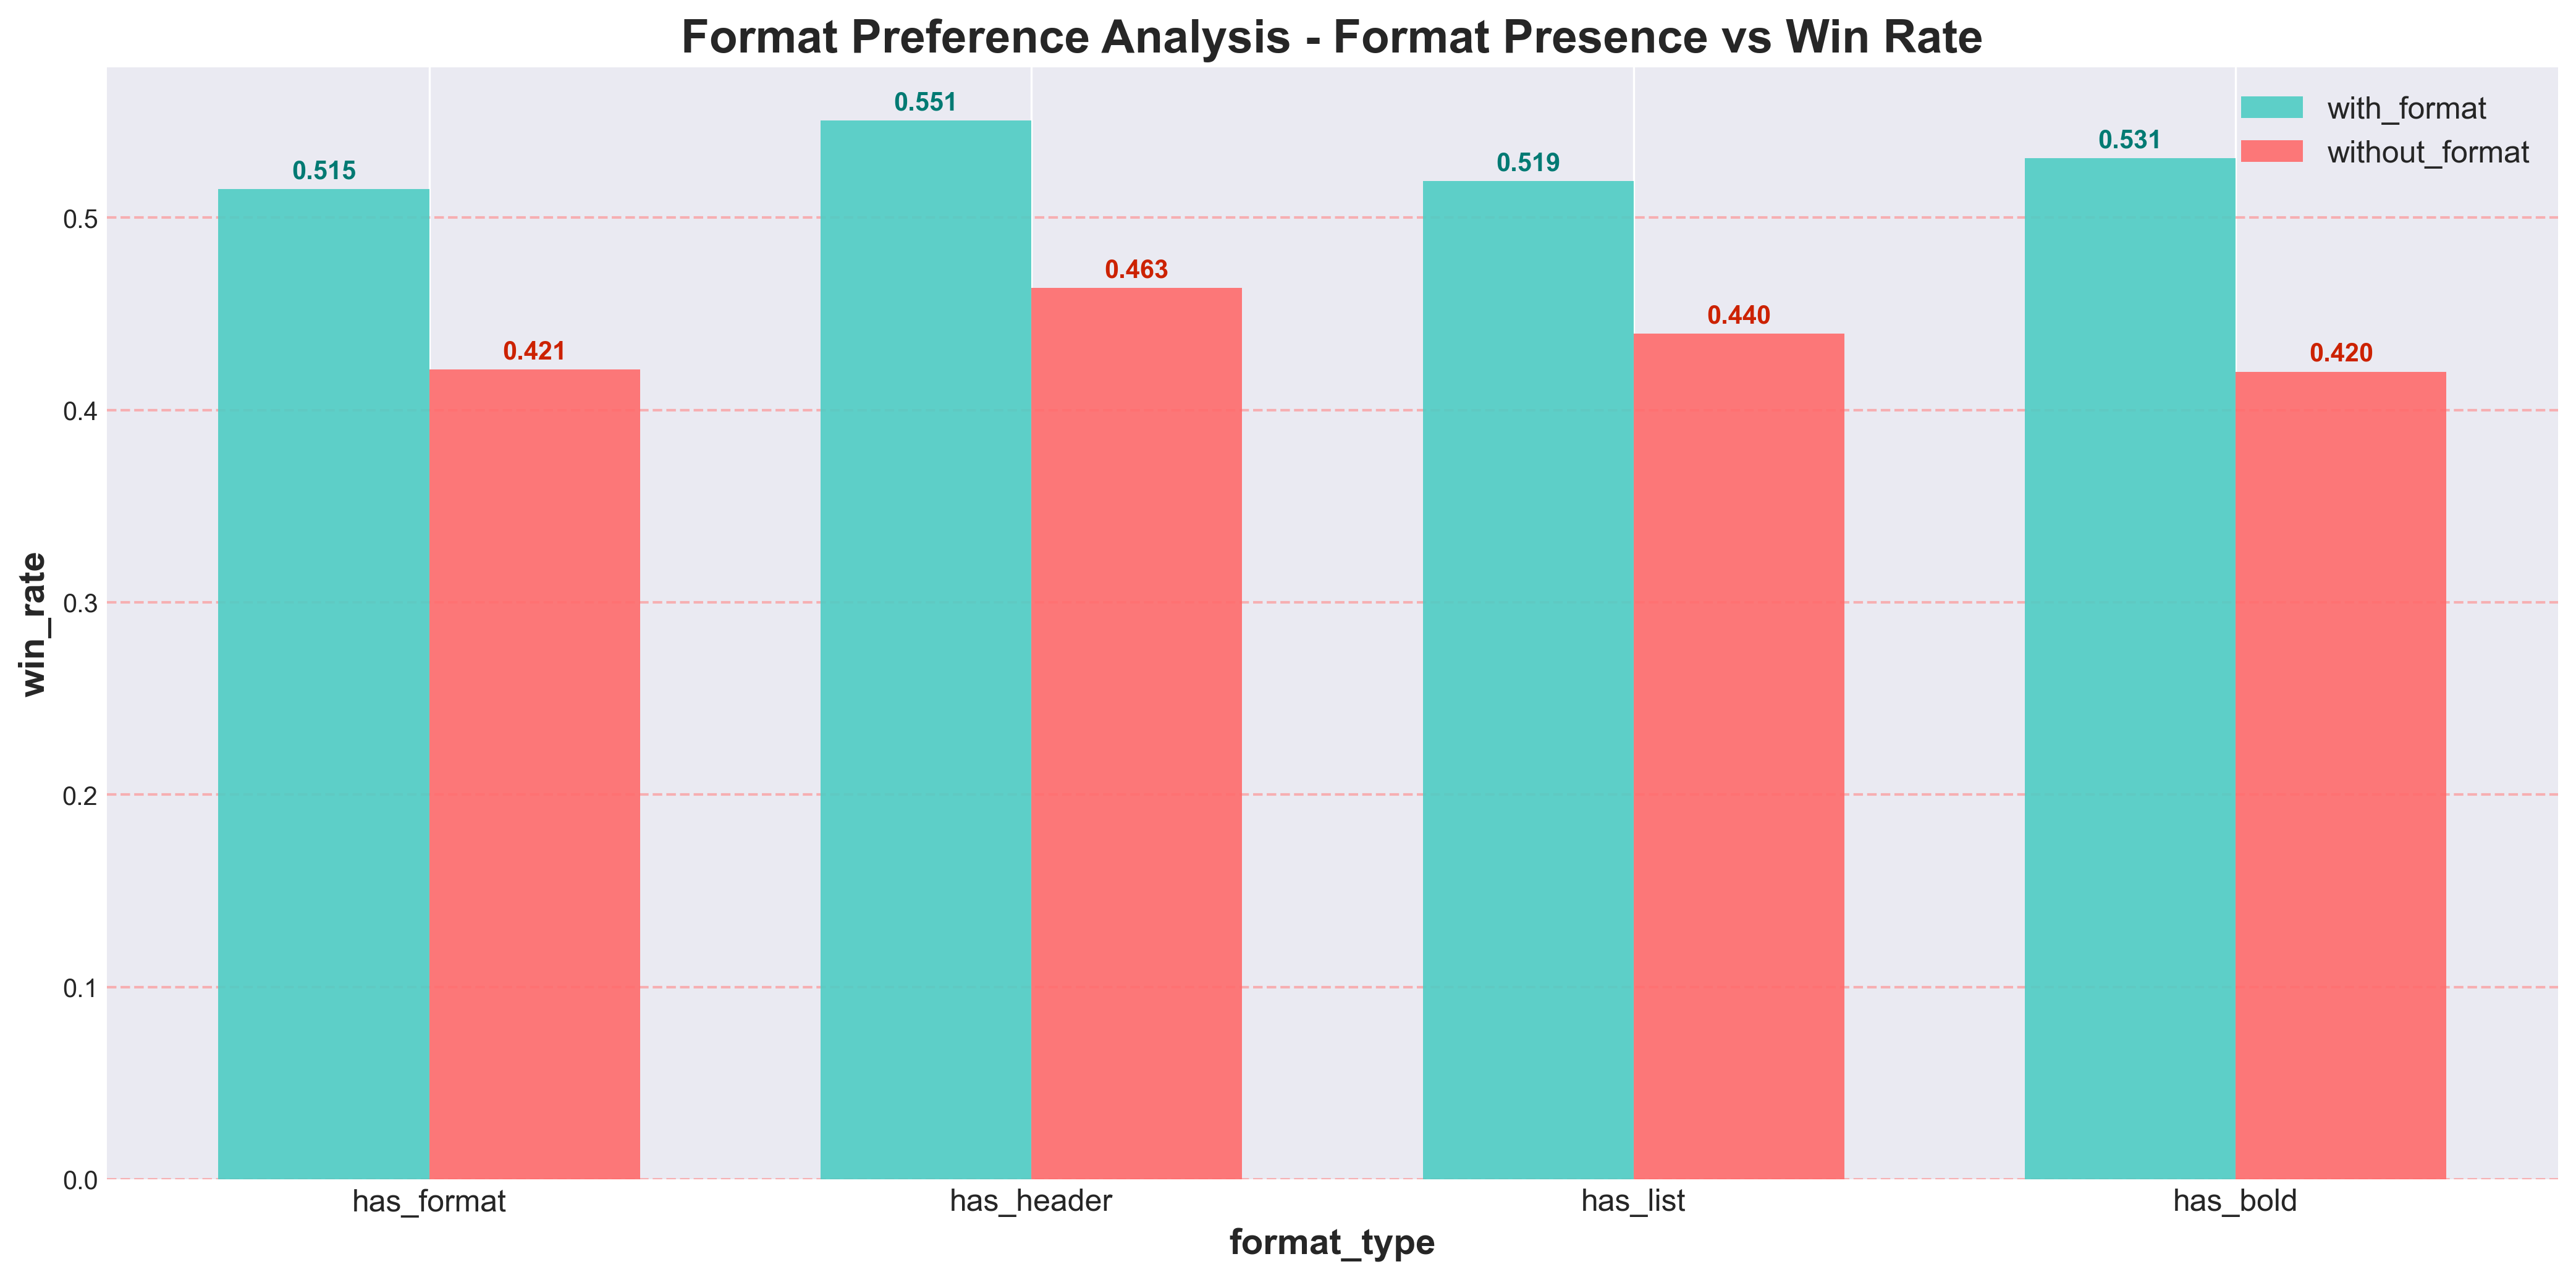
\includegraphics[width=0.9\textwidth]{figures/P05_01_format_presence_bar_chart.png}
\caption{格式存在性与胜率的关联}
\label{fig:format_presence}
\end{figure}

注：图 \ref{fig:format_presence} 比较包含对应格式元素与不包含对应格式元素的回答胜率差异，用于展示标题、列表和粗体在存在性层面的总体关联。

\begin{figure}[htbp]
\centering
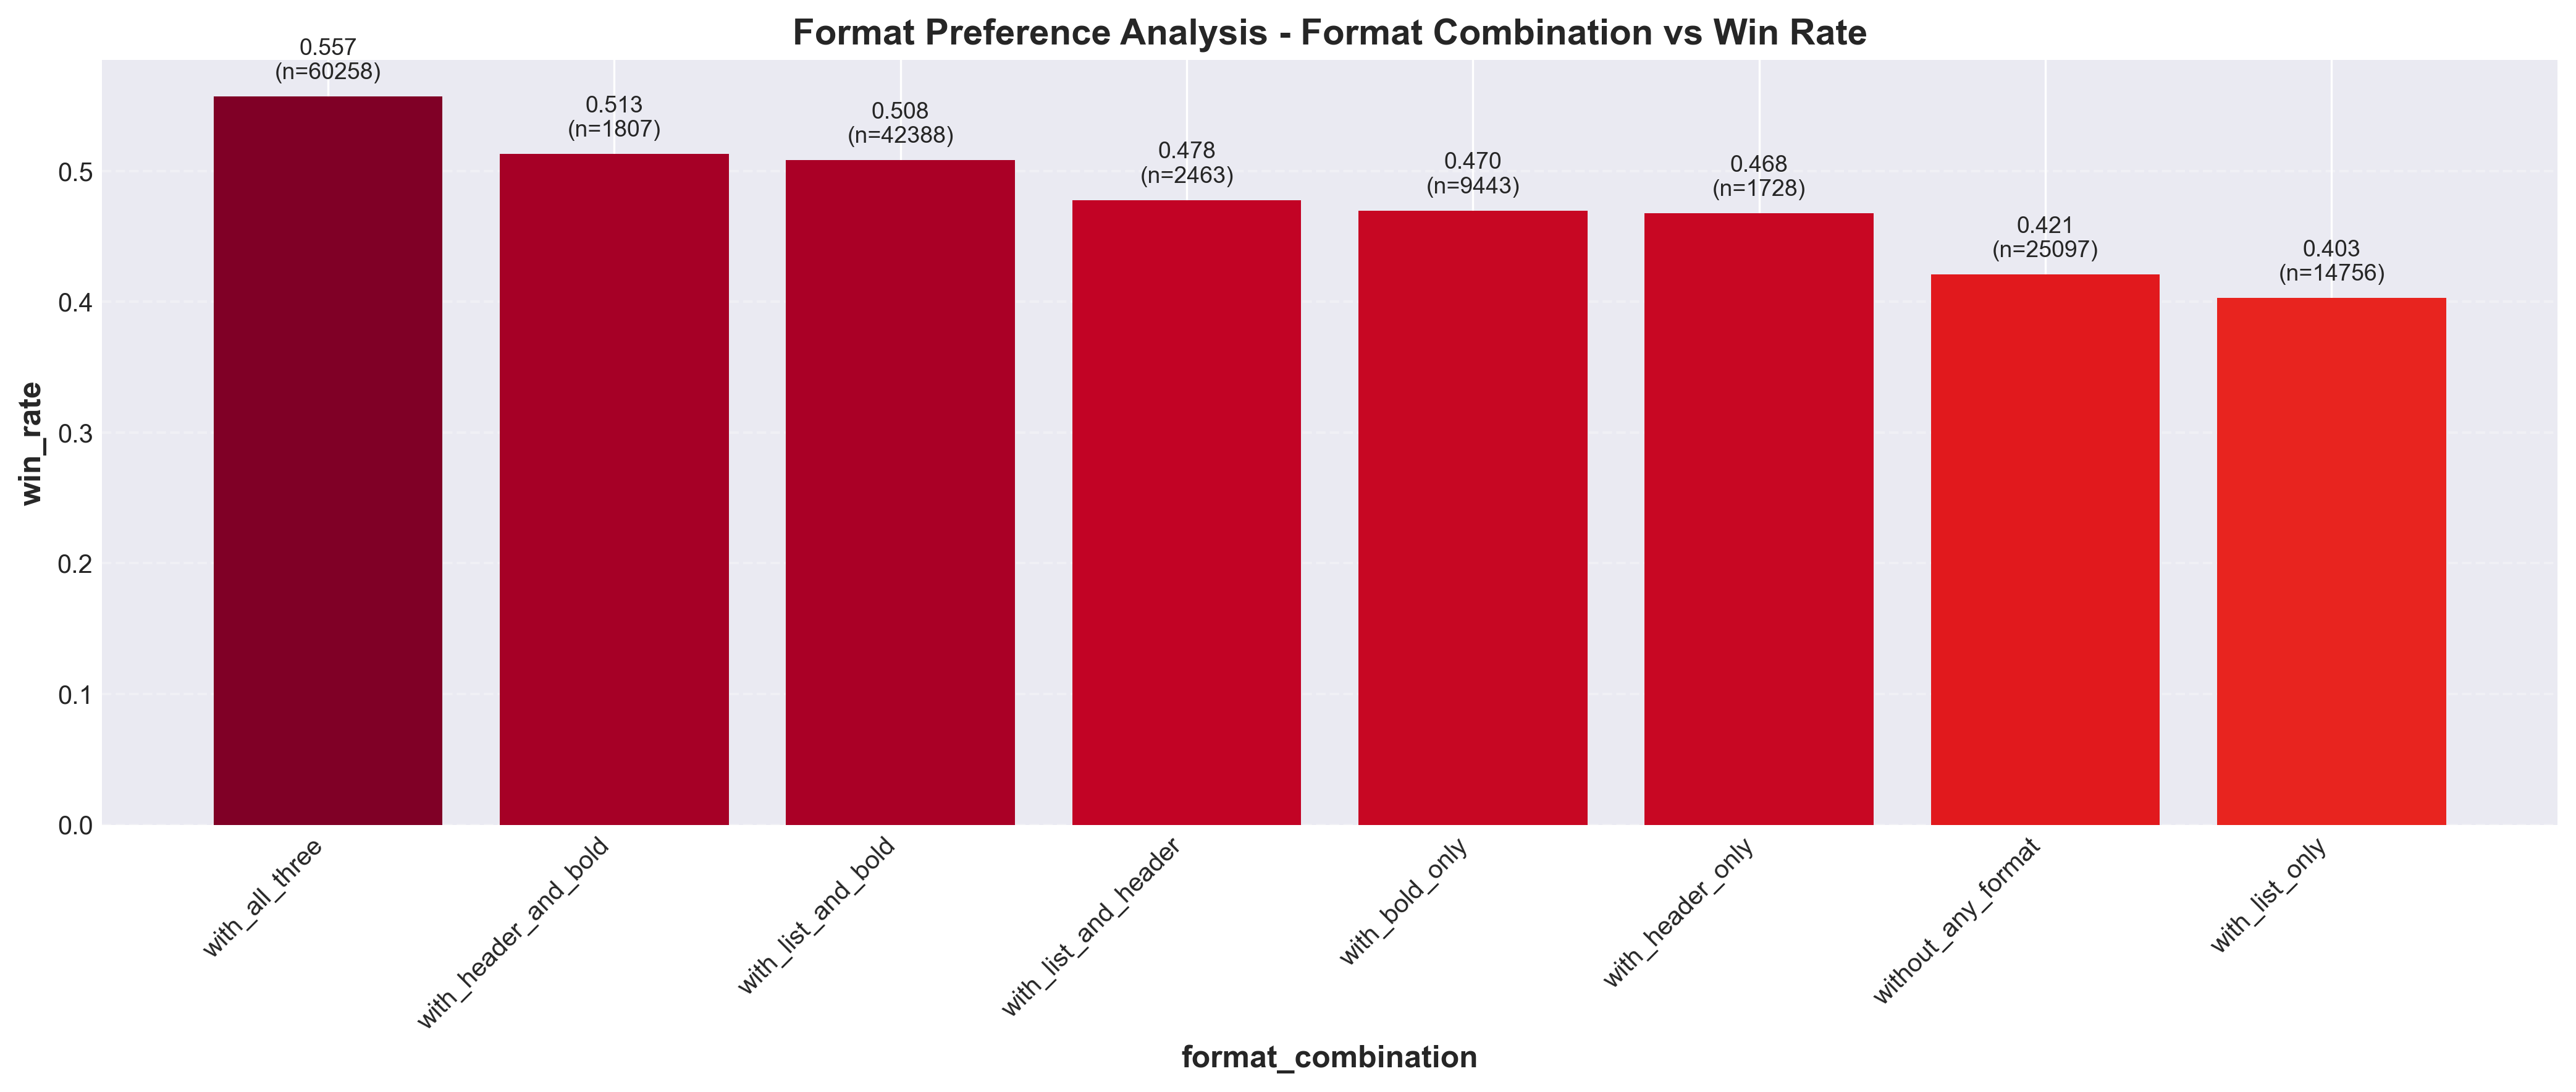
\includegraphics[width=0.9\textwidth]{figures/P05_05_format_combination_bar_chart.png}
\caption{格式组合与胜率的关联}
\label{fig:format_combination}
\end{figure}

注：图 \ref{fig:format_combination} 用于展示多种格式特征共同出现时的胜率差异，其解释重点在于组合模式的描述，而不是对单一格式变量作独立效应判断。

\subsection{长度偏好的正式统计检验}
在正式检验层面，本文对满足最小样本要求的 13 个子集进行了单侧 Wilcoxon 符号秩检验，并采用 Bonferroni 校正控制多重比较。对应的校正阈值为 \(\alpha' = 0.05/13 = 0.0038\)。结果显示，13 个有效子集中有 12 个在校正后仍显著，仅“创意+指令+代码”子集不显著。全量样本的 rank-biserial \(r\) 为 0.3362，属于中等效应区间；无类别子集效应量相对较低（\(r=0.3155\)），而数学子集（\(r=0.3837\)）、代码子集（\(r=0.3529\)）和仅指令遵循子集（\(r=0.3458\)）的效应量高于全量，其中数学加代码复合子集的效应量最高（\(r=0.4101\)）。这一模式说明，不同任务场景对长度偏好的强化程度存在明显异质性；在无任务标签的通用对话中，效应相对偏弱，而在代码、数学等对回答完整度有较高要求的场景中，效应更为突出。

这一结果表明，长度偏好并不是只体现在平均值差异上，而是在配对比较与秩统计意义下都有稳定方向性。这样一来，H1 在存在性检验层面获得了明确支持。

本文采用单侧 Wilcoxon 的理论依据在于，研究问题本身有明确方向性，即检验“胜者是否系统性更长”，而不是仅检验“长度差是否不为 0”。Bonferroni 校正用来避免多子集并行检验时过度报告显著性；rank-biserial \(r\) 则负责把“显著”转化为“差异量级”。在本研究采用的常用阈值下，\(0.1<r<0.3\) 可以视为小效应，\(0.3<r<0.5\) 可以视为中等效应，\(r>0.5\) 可以视为大效应；这样一来，全量样本 \(r=0.3362\) 可归入中等效应。中位长度差的 Bootstrap 区间基于 1000 次重采样计算，进一步说明长度优势并不是由少量极端长回答拉动，而是在配对层面呈现出稳定的整体偏移。

\begin{longtable}{lrlrrrr}
\caption{长度偏好正式统计检验结果汇总}\\
\toprule
子集 & 中位长度差 & 95\%置信区间 & 校正后\(p\)值 & rank-biserial \(r\) & Cohen's \(d\) & Hedges' \(g\) \\
\midrule
\endfirsthead
\toprule
子集 & 中位长度差 & 95\%置信区间 & 校正后\(p\)值 & rank-biserial \(r\) & Cohen's \(d\) & Hedges' \(g\) \\
\midrule
\endhead
数字+代码 & 97.5 & \([+52.5,+148.0]\) & \(<0.001\) & 0.410 & 0.144 & 0.144 \\
指令+数字+代码 & 139 & \([+60.0,+229.0]\) & \(<0.001\) & 0.407 & 0.117 & 0.117 \\
创意+指令+代码 & 47 & \([-64.0,+209.0]\) & 0.517 & 0.405 & 0.185 & 0.184 \\
仅数字 & 56 & \([+45.0,+72.0]\) & \(<0.001\) & 0.384 & 0.153 & 0.153 \\
指令+数字 & 129 & \([+79.0,+186.0]\) & \(<0.001\) & 0.380 & 0.104 & 0.103 \\
创意+代码 & 74.5 & \([-4.0,+140.5]\) & 0.003 & 0.371 & 0.168 & 0.168 \\
仅代码 & 203 & \([+189.0,+218.0]\) & \(<0.001\) & 0.353 & 0.190 & 0.190 \\
创意+指令 & 77.5 & \([+44.5,+116.0]\) & \(<0.001\) & 0.349 & 0.189 & 0.189 \\
仅指令遵循 & 121.5 & \([+99.0,+140.5]\) & \(<0.001\) & 0.346 & 0.168 & 0.168 \\
仅创意写作 & 60 & \([+50.0,+69.0]\) & \(<0.001\) & 0.345 & 0.223 & 0.223 \\
指令+代码 & 256 & \([+217.0,+285.0]\) & \(<0.001\) & 0.337 & 0.183 & 0.183 \\
全量 & 125 & \([+121.0,+130.0]\) & \(<0.001\) & 0.336 & 0.181 & 0.181 \\
无类别 & 121 & \([+115.0,+126.0]\) & \(<0.001\) & 0.316 & 0.218 & 0.218 \\
\bottomrule
\end{longtable}

\subsection{格式偏好的正式统计检验}
格式偏好的正式检验同样采用 Wilcoxon 框架，但对每个子集同时比较标题、列表和粗体三类格式特征，并在子集内进行 Bonferroni 校正。结果显示，若只看格式计数差，绝大多数主要子集中的三类格式都能达到显著；全量样本中，标题的 rank-biserial \(r\) 为 0.3960，列表为 0.3833，粗体为 0.3696，三类效应量均处于中等水平，说明偏好差异并不是仅靠大样本量放大的微弱信号。但引入密度辅助检验后，标题和粗体的信号更稳定，而列表的密度信号在全量样本中不显著，在多个子集中也不稳定。

这样一来，格式偏好不能被理解为“所有格式都同样有利”。更精确的表述为：结构化格式作为整体与偏好存在关联，但真正较稳定的独立格式信号主要集中在标题和粗体两类变量上，而列表更接近长度扩张或文本组织方式的伴生结果。H2 因而得到部分支持，并为后续稳健性分析提供了方向。

本文将“格式计数差检验”作为主检验，将“格式密度差检验”作为辅助检验。前者回答的是“胜者是否使用了更多格式元素”，后者回答的是“在控制文本长度规模之后，这种格式优势是否仍然也能看出”。正因为这两个问题并不完全相同，列表在计数层面显著、但在密度层面不显著这一结果才有解释价值：它说明部分格式差异并不构成独立偏好，而只是更长文本和更复杂组织方式自然带来的副产物。

\begin{longtable}{llrrrrr}
\caption{格式偏好正式统计检验结果汇总}\\
\toprule
子集 & 格式特征 & 95\%置信区间 & 校正后\(p\)值 & rank-biserial \(r\) & 中位密度差 \\
\midrule
\endfirsthead
\toprule
子集 & 格式特征 & 95\%置信区间 & 校正后\(p\)值 & rank-biserial \(r\) & 中位密度差 \\
\midrule
\endhead
创意+指令+代码 & 粗体 & \([+0.0,+1.0]\) & 0.973 & 0.473 & 0 \\
创意+指令+代码 & 标题 & \([+0.0,+0.0]\) & 1 & 0.469 & 0 \\
创意+指令+代码 & 列表 & \([+0.0,+0.0]\) & 1 & 0.498 & 0 \\
指令+数学+代码 & 粗体 & \([+0.0,+1.0]\) & 0.008 & 0.430 & 0.032 \\
指令+数学+代码 & 标题 & \([+0.0,+0.0]\) & 0.079 & 0.447 & 0 \\
指令+数学+代码 & 列表 & \([+0.0,+3.0]\) & 0.073 & 0.452 & -0.0002 \\
指令+代码 & 粗体 & \([+0.0,+1.0]\) & \(<0.001\) & 0.426 & 0 \\
指令+代码 & 标题 & \([+0.0,+0.0]\) & \(<0.001\) & 0.453 & 0 \\
指令+代码 & 列表 & \([+0.0,+2.0]\) & \(<0.001\) & 0.433 & -0.0002 \\
指令+数学 & 粗体 & \([+1.0,+4.0]\) & \(<0.001\) & 0.382 & 0.0007 \\
指令+数学 & 标题 & \([+0.0,+0.0]\) & 0.439 & 0.475 & 0 \\
指令+数学 & 列表 & \([+0.0,+3.0]\) & 0.002 & 0.434 & 0 \\
创意+指令 & 粗体 & \([+0.0,+0.0]\) & \(<0.001\) & 0.430 & 0.324 \\
创意+指令 & 标题 & \([+0.0,+0.0]\) & 0.021 & 0.440 & 0.335 \\
创意+指令 & 列表 & \([+0.0,+0.0]\) & \(<0.001\) & 0.421 & 0 \\
数学+代码 & 粗体 & \([+0.0,+1.5]\) & \(<0.001\) & 0.421 & 0 \\
数学+代码 & 标题 & \([+0.0,+0.0]\) & \(<0.001\) & 0.422 & 0 \\
数学+代码 & 列表 & \([+0.0,+2.0]\) & 0.004 & 0.442 & \(<0.0001\) \\
创意+代码 & 粗体 & \([+0.0,+1.0]\) & 0.088 & 0.425 & 0 \\
创意+代码 & 标题 & \([+0.0,+0.0]\) & 0.397 & 0.447 & 0 \\
创意+代码 & 列表 & \([+0.0,+0.5]\) & 0.02 & 0.397 & 0 \\
仅指令遵循 & 粗体 & \([+0.0,+1.0]\) & \(<0.001\) & 0.388 & 0 \\
仅指令遵循 & 标题 & \([+0.0,+0.0]\) & \(<0.001\) & 0.429 & 0 \\
仅指令遵循 & 列表 & \([+0.0,+0.0]\) & \(<0.001\) & 0.407 & 0 \\
仅代码 & 粗体 & \([+2.0,+2.0]\) & \(<0.001\) & 0.4 & 0.0003 \\
仅代码 & 标题 & \([+0.0,+0.0]\) & \(<0.001\) & 0.398 & 0 \\
仅代码 & 列表 & \([+2.0,+2.0]\) & \(<0.001\) & 0.412 & \(<0.0002\) \\
仅数字 & 粗体 & \([+1.0,+1.0]\) & \(<0.001\) & 0.368 & 0.0007 \\
仅数字 & 标题 & \([+0.0,+0.0]\) & \(<0.001\) & 0.438 & 0 \\
仅数字 & 列表 & \([+0.0,+1.0]\) & \(<0.001\) & 0.389 & 0 \\
仅创意写作 & 粗体 & \([+0.0,+0.0]\) & \(<0.001\) & 0.393 & 0 \\
仅创意写作 & 标题 & \([+0.0,+0.0]\) & \(<0.001\) & 0.410 & \(<0.001\) \\
仅创意写作 & 列表 & \([+0.0,+0.0]\) & \(<0.001\) & 0.376 & 0 \\
全量 & 粗体 & \([+1.0,+1.0]\) & \(<0.001\) & 0.370 & \(<0.001\) \\
全量 & 标题 & \([+0.0,+0.0]\) & \(<0.001\) & 0.396 & 0 \\
全量 & 列表 & \([+0.0,+1.0]\) & \(<0.001\) & 0.383 & 0 \\
无类别 & 粗体 & \([+2.0,+2.0]\) & \(<0.001\) & 0.342 & 0.0005 \\
无类别 & 标题 & \([+0.0,+0.0]\) & \(<0.001\) & 0.371 & 0 \\
无类别 & 列表 & \([+1.0,+2.0]\) & \(<0.001\) & 0.354 & 0 \\
\bottomrule
\end{longtable}

% ==================== 第六章 ====================
\section{净效应估计与稳健性验证}

\subsection{嵌套逻辑回归下的净效应分解}
为了识别长度和格式偏好中有多少属于控制混淆后仍保留的净效应，本文采用了嵌套逻辑回归。首先看前置验证结果，模型胜率与平均 token 数的 Spearman 相关为 0.7171，与平均格式数的相关为 0.5318。这也说明模型能力与长度、格式风格之间存在明显共线性，这样一来，将 \ability、\verbosity 和 \formatt 纳入控制，是识别净效应的必要前提。

本文采用分层推进的嵌套设计，而非一次性投入全部变量。长度模型的 M0 只估计粗长度效应，M1 加入问题特征，M2 进一步加入 quality criteria，M3 再加入模型能力与风格代理变量；格式模型的 F0 到 F3 采用同样思路，并始终把 \tokendiff 作为固定协变量纳入。这样设计的价值在于，可以直接观察核心 OR 如何随控制项扩展而变化：如果某个效应在加入控制后快速衰减，就说明它更可能受到混淆放大；如果控制后仍保持稳定，则更接近独立净效应。

在长度模型中，全量样本的 z\_\tokendiff 粗效应 OR 为 1.9045；加入问题特征与质量维度后变化很小；加入模型能力和风格后，M3 的净效应 OR 下降为 1.3551。按照本文的定义，混淆比例按 \(1-(\mathrm{OR}_{M3}-1)/(\mathrm{OR}_{M0}-1)\) 计算，即 \(1-(1.3551-1)/(1.9045-1)=60.74\%\)。这也说明原始长度粗效应中，约 61\% 可由任务类型、质量维度以及模型能力与风格差异解释，剩余约 39\% 为长度的独立净效应。这样也能看出，长度优势确实被模型层因素显著放大，但并没有在控制后消失。

进一步看全量样本 M3 的附加指标，AME 为 0.0760，Wald \(r\) 为 0.0817。这也说明在控制一系列问题层和模型层因素后，长度差每提高一个标准化单位，A 侧获胜概率平均仍会出现正向变化，但其强度已经明显低于粗模型阶段。长度效应并未消失，而是从“偏强的粗关联”收缩为“仍可检测到的净关联”；这也是本文强调“长度优势存在，但不能简单等同于长度本身因果作用”的原因。

在格式模型中，全量样本控制长度后，标题密度差、列表密度差和粗体密度差的粗格式效应 OR 分别为 1.1133、0.9398 和 1.1570。进一步控制问题特征、质量维度及模型能力和风格后，F3 中标题密度差净 OR 为 1.0606，粗体密度差净 OR 为 1.0855，列表密度差净 OR 仅为 1.0249，且其混淆比例高达 \(141.31\%\)。对照来看，标题和粗体的混淆比例分别为 \(46.47\%\) 和 \(45.55\%\)，说明控制混淆后约一半粗效应仍然保留。这也说明标题和粗体存在较弱但稳定的独立作用，而列表主要呈现混淆驱动特征。

混淆比例表示粗效应被控制变量解释掉的程度。当混淆比例接近 \(0\%\) 时，说明控制变量对原始结论影响较小；当混淆比例接近或超过 \(100\%\) 时，则说明粗效应几乎完全由控制项解释，甚至方向都可能发生反转。列表密度的结果正体现了这一点，因而它不适合与标题、粗体并列写入主结论。

\begin{figure}[htbp]
\centering
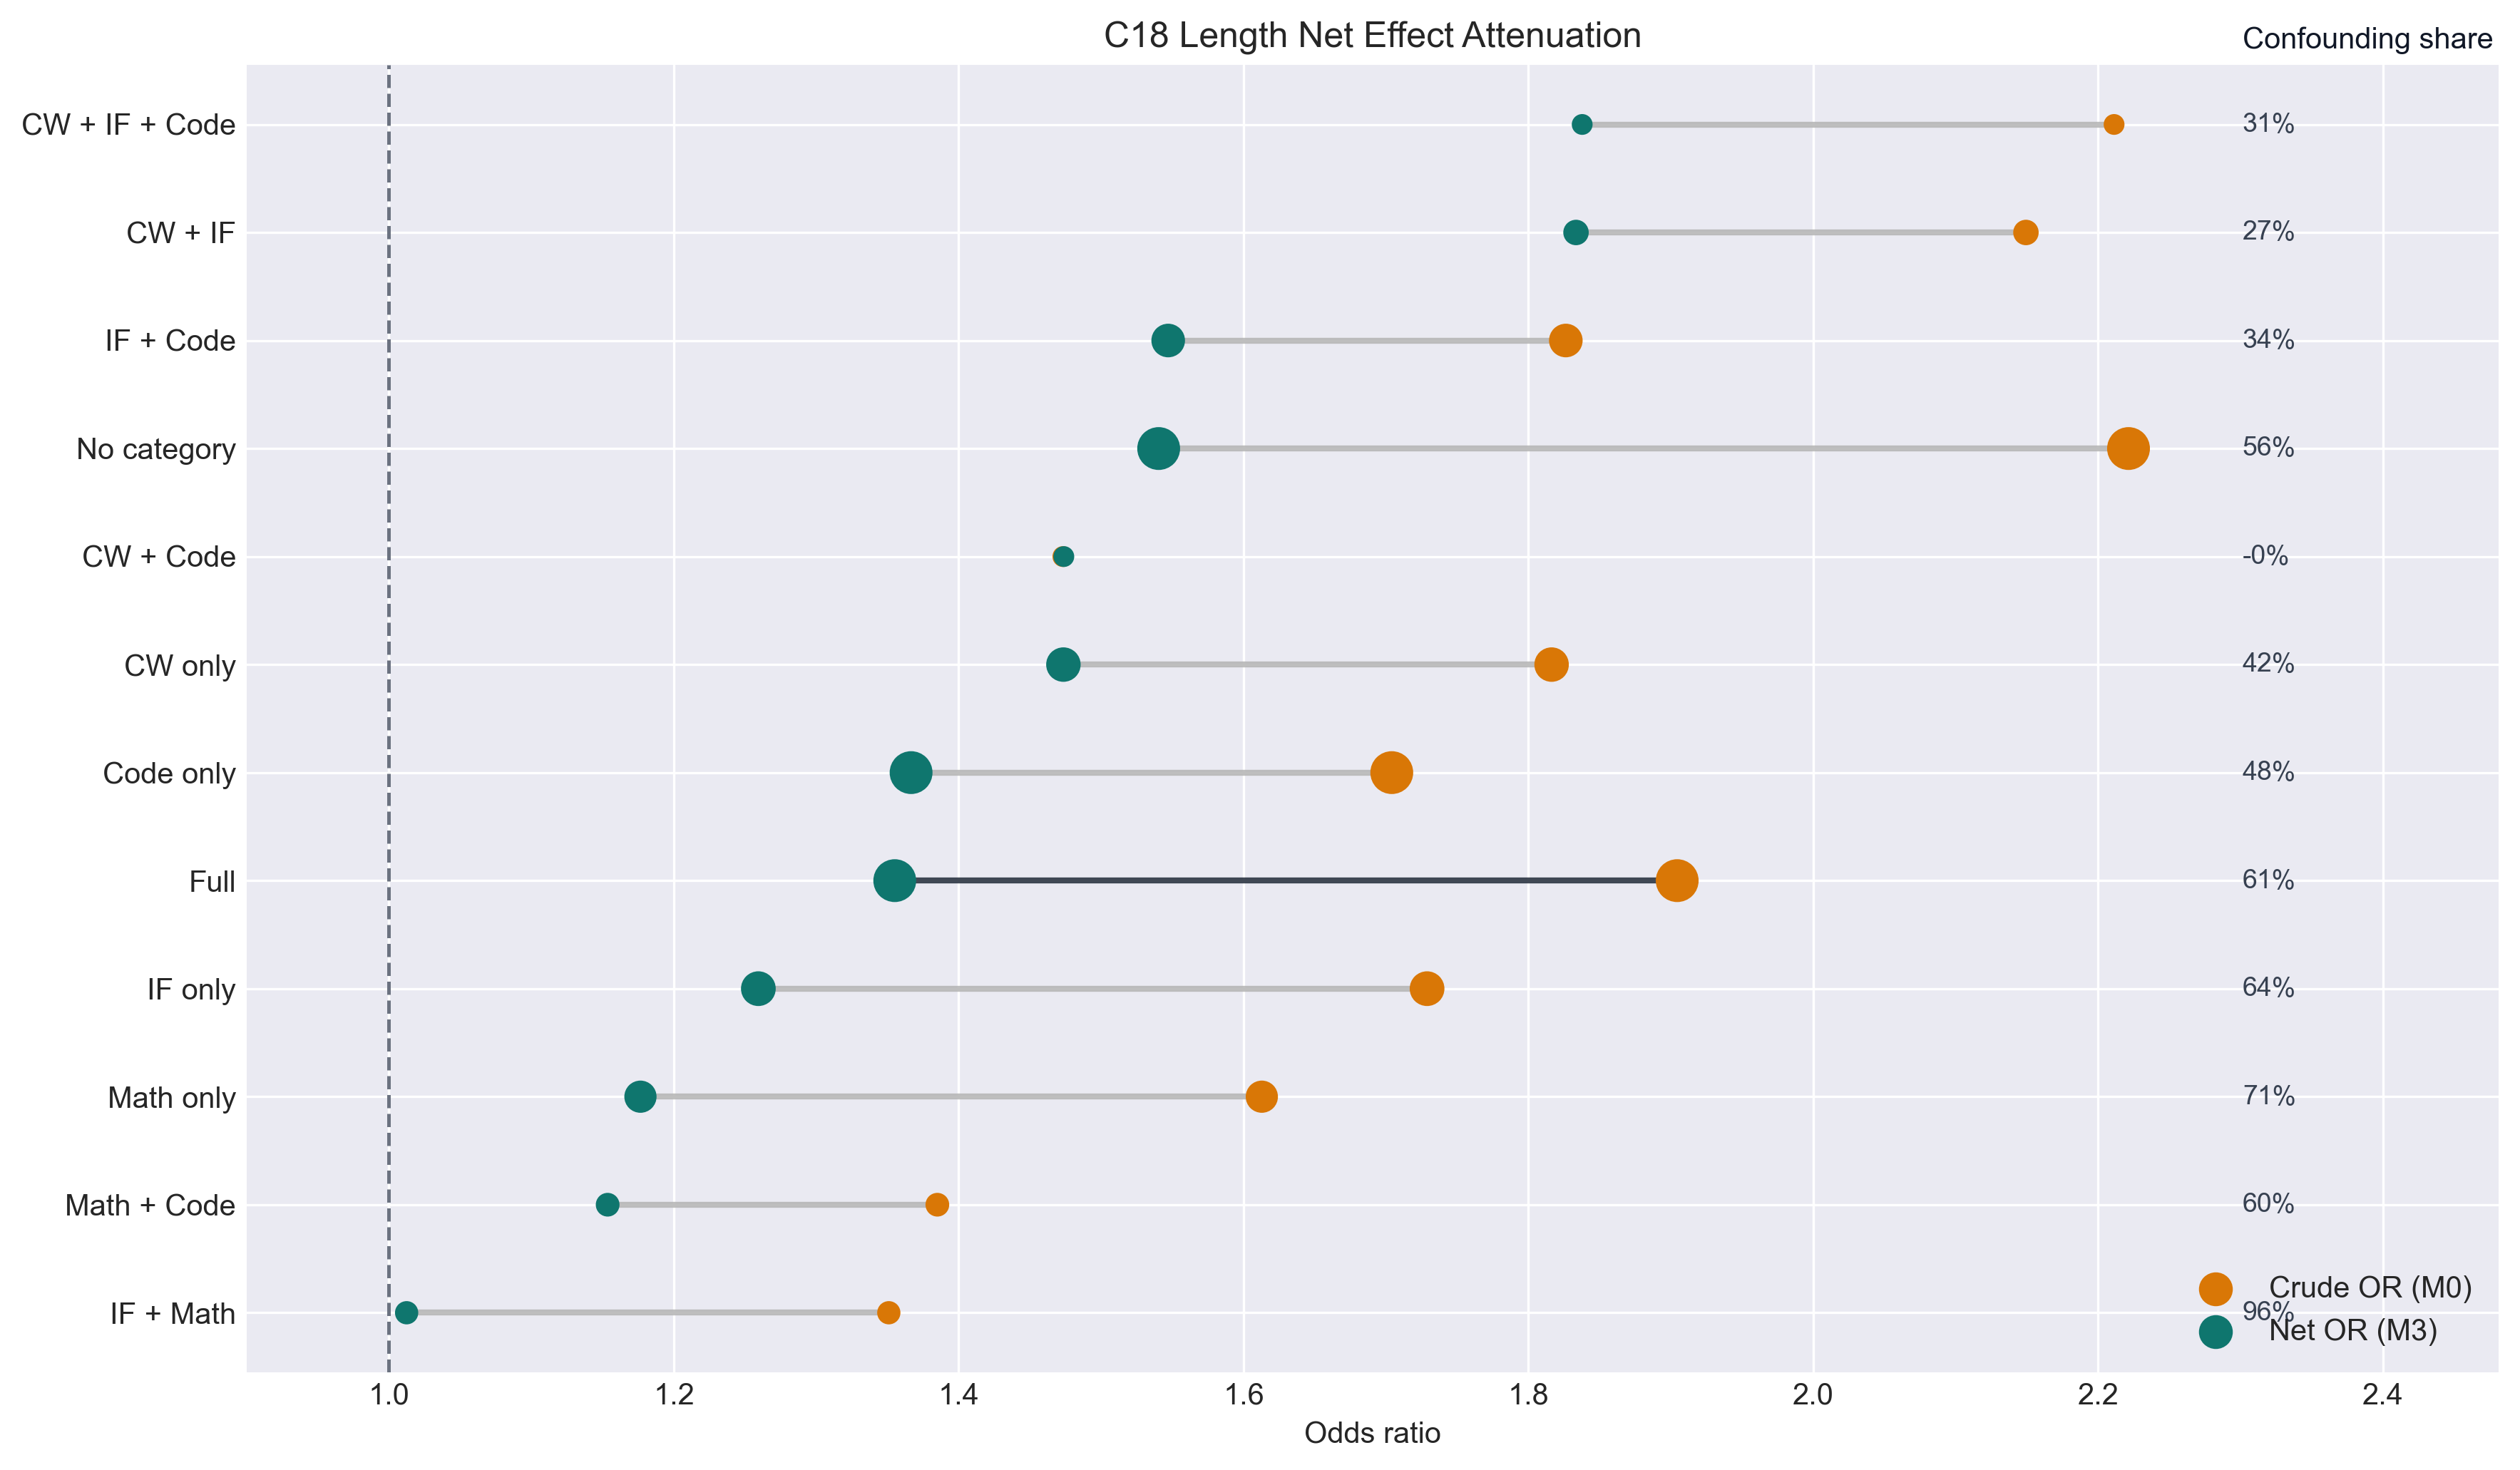
\includegraphics[width=0.9\textwidth]{figures/P08_length_confounding_attenuation.png}
\caption{长度净效应衰减图}
\label{fig:length_attenuation}
\end{figure}

\begin{figure}[htbp]
\centering
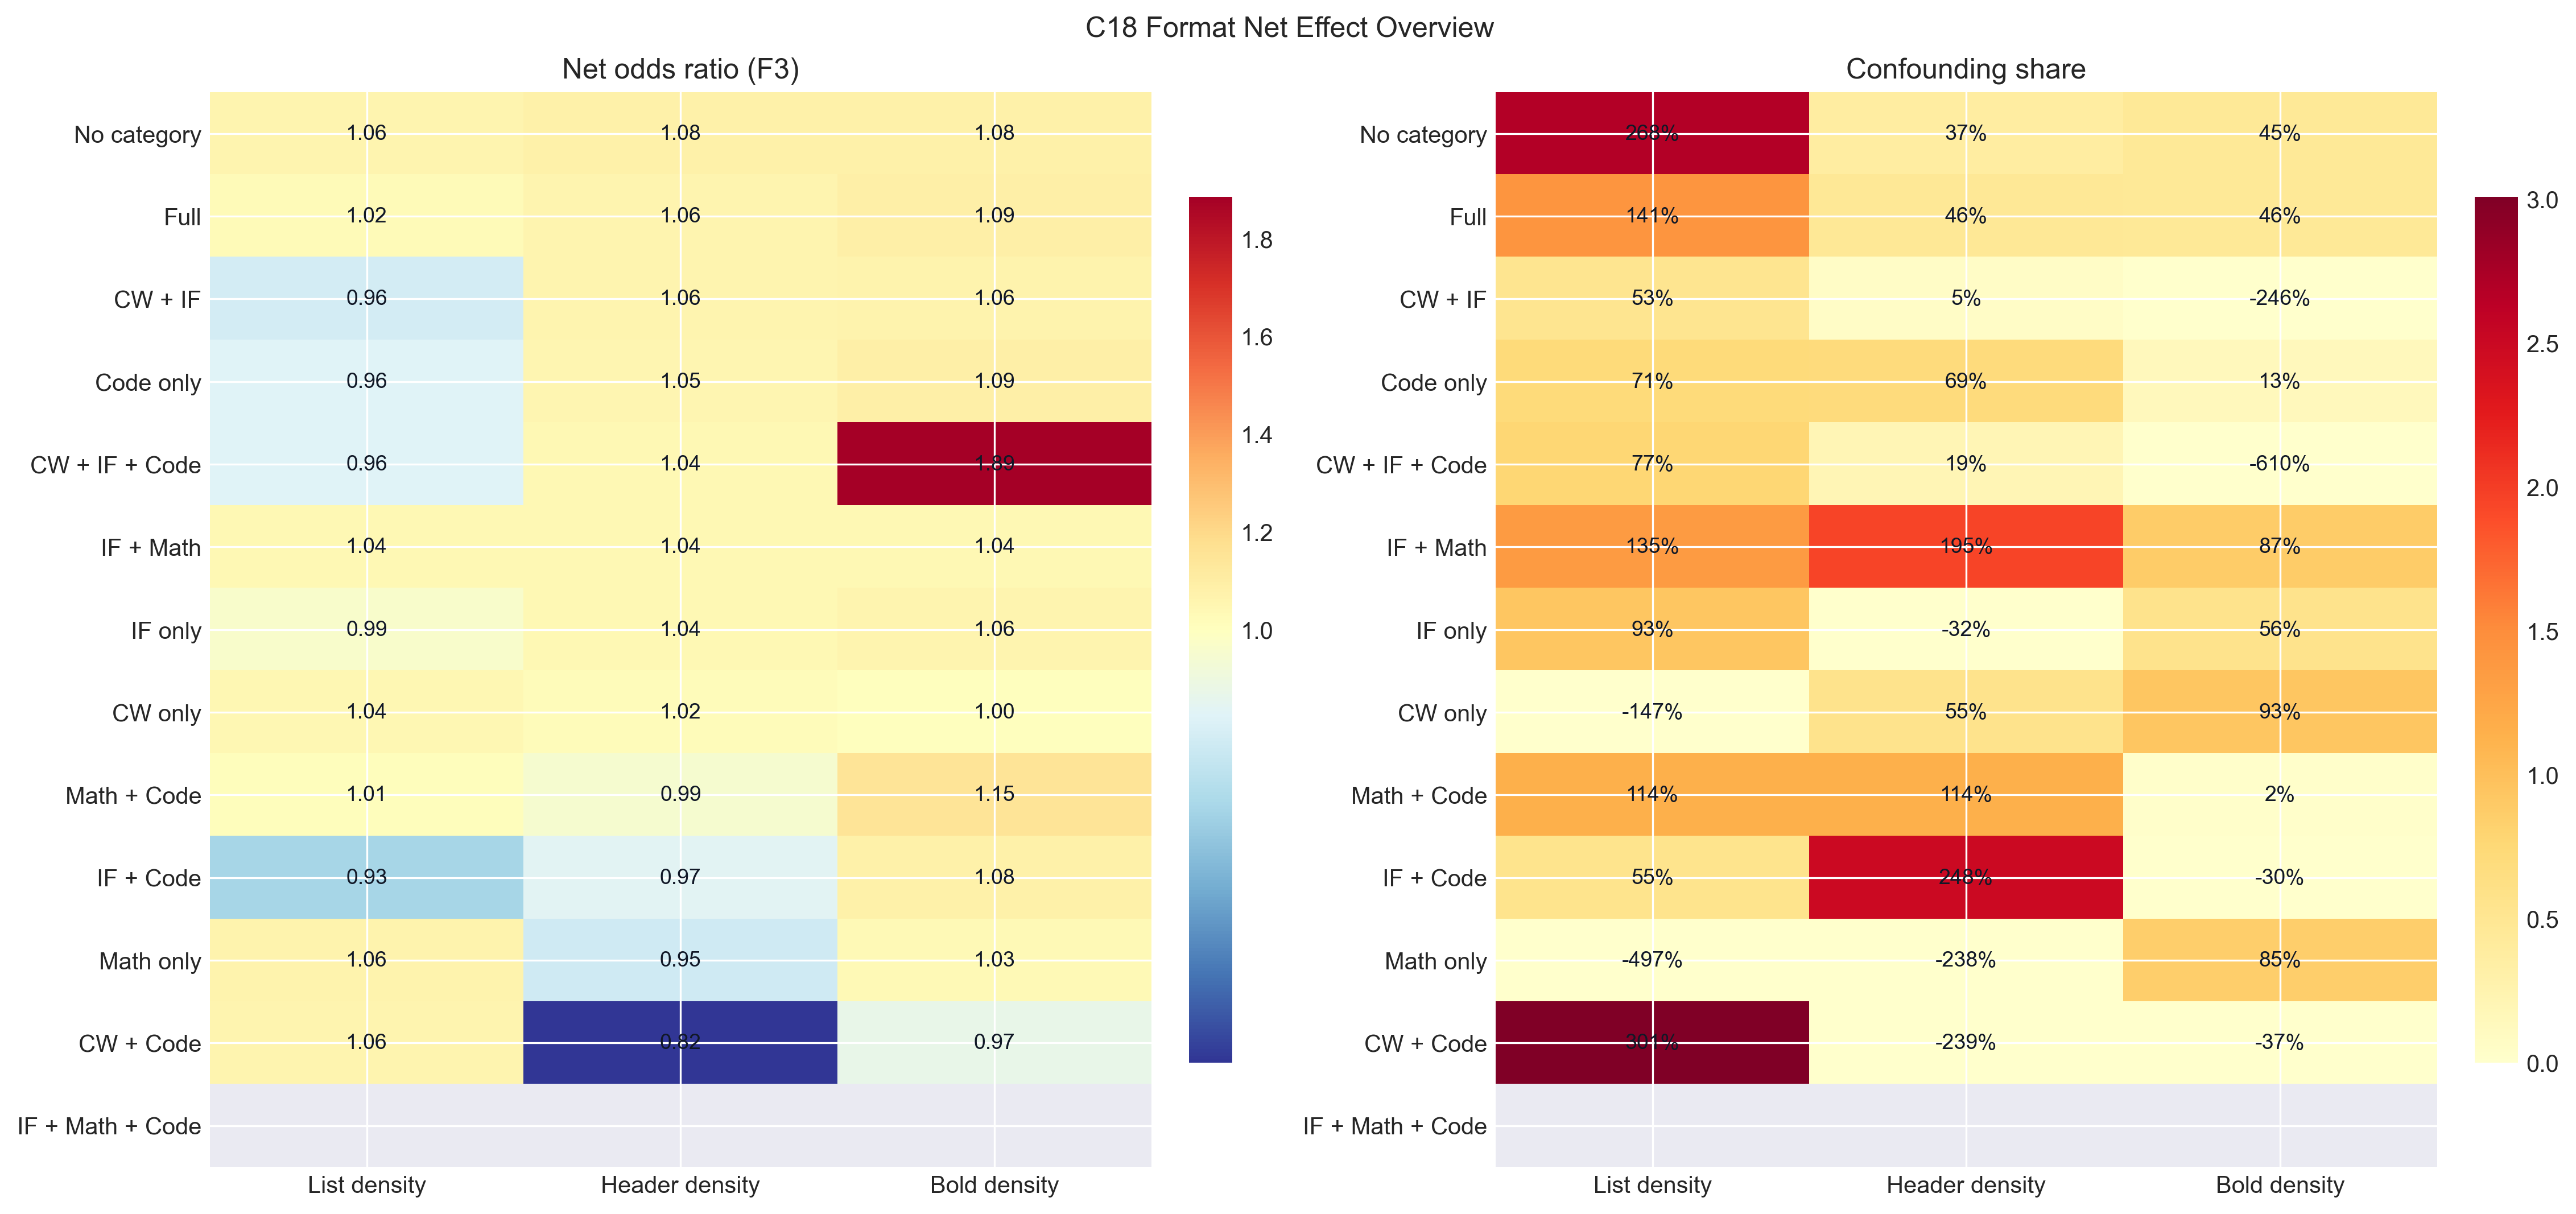
\includegraphics[width=0.9\textwidth]{figures/P09_format_net_effect_heatmaps.png}
\caption{格式偏好检验汇总图}
\label{fig:format_summary}
\end{figure}

\subsection{调整逻辑回归与 IPW 稳健性验证}
为避免结论依赖单一建模框架，本文还进一步采用调整逻辑回归和稳定化 IPW。对于长度效应，全量样本在剔除长度平局后保留 78,783 条记录，更长一侧获胜比例为 0.6236。粗模型 OR 为 2.7446，调整模型 OR 为 1.9103，IPW ATE 为 0.1489，95\% 置信区间为 \([0.1351,0.1614]\)。这也说明了，在处理效应视角下，长度优势仍然显著存在。

这一部分与前面的净效应模型在识别语义上并不完全相同。调整逻辑回归回答的是“在控制观测协变量后，处理变量与结果之间是否仍呈稳定关联”；IPW 则尝试在观测协变量平衡后的伪总体中估计“如果把处理组和对照组放在同一背景分布下，处理平均会让结果增加多少”。这样一来，OR 和 ATE 不能简单互相替代。OR 描述的是赔率变化，ATE 描述的是概率层面的平均变化。两者方向一致、且 IPW 区间不跨 0，才构成更强的稳健性证据。

对于格式效应，标题密度主分析的全量样本中，调整模型 OR 为 1.1317，IPW ATE 为 0.0277，95\% 置信区间为 \([0.0221,0.0358]\)；粗体密度的全量调整模型 OR 为 1.1060，IPW ATE 为 0.0246，95\% 置信区间为 \([0.0165,0.0379]\)。对照来看，列表密度在全量样本中的辅助密度检验已不显著，在稳健性分析中也未被纳入主结论，只保留为敏感性变量。

本文在 IPW 中还同时关注倾向得分范围和 ESS。前者用来避免极端权重，后者用来判断加权后是否只剩少量样本在“支撑结论”。就全量长度分析而言，倾向得分被截断在 \([0.0100,0.9900]\)，ESS 为 20592.0，说明虽然加权会降低有效样本量，但结果并不是由极少数异常样本支撑起来的。格式分析中同样保留这一检查逻辑，从而避免仅凭显著结果做出过度解释。

稳健性结果说明，H3 在全量样本层面得到了明确支持，但不同任务子集存在明显异质性。例如，仅创意写作子集调整 OR 为 1.9939、IPW ATE 为 0.1755；仅代码子集调整 OR 为 1.7755、IPW ATE 为 0.1562；而仅数字子集调整 OR 仅为 1.3403、IPW ATE 为 0.0717。数学场景的长度净效应明显偏弱，与嵌套回归中数字子集混淆比例高达 \(71.19\%\) 的发现相互印证。格式效应同样受任务语境影响，在部分创意写作、代码子集中的标题或粗体稳健性差异更为有限。

\begin{table}[htbp]
\centering
\caption{长度与格式稳健性结果汇总}
\label{tab:robustness}
\begin{tabular}{lllll}
\toprule
特征 & 分析角色 & 样本量 & 调整 OR [95\% CI] & IPW ATE [95\% CI] \\
\midrule
长度差 / \longer & 主分析 & 78,783 & 1.910 [1.842, 1.982] & 0.149 [0.135, 0.161] \\
标题密度 & 主分析 & 49,092 & 1.132 [1.083, 1.182] & 0.028 [0.022, 0.036] \\
粗体密度 & 主分析 & 70,193 & 1.106 [1.064, 1.149] & 0.025 [0.017, 0.038] \\
列表密度 & 敏感性分析 & 69,305 & 1.026 [0.992, 1.062] & 0.002 [-0.005, 0.009] \\
\bottomrule
\end{tabular}
\end{table}

注：表 \ref{tab:robustness} 中“净效应”对应控制混淆后的回归 OR，“处理效应”对应 IPW 框架下的 ATE。二者刻画对象不同，不宜直接比较数值大小；列表密度仅作为敏感性分析保留。

\subsection{倾向得分匹配与平衡性诊断}
除了加权估计之外，本文还采用 1:1 最近邻倾向得分匹配，并以标准化均值差作为平衡性指标。全量样本中，共匹配 39,237 对，treated match rate 为 \(100\%\)，公共支持区间覆盖率为 \(100\%\)。匹配前 \(\max[\mathrm{SMD}]\) 为 1.4732，mean\([\mathrm{SMD}]\) 为 0.2502；匹配后分别降至 0.1765 和 0.0597，说明样本可比性显著改善。

在具体实现上，本文使用的是按 \(\mathrm{logit}(\mathrm{PS})\) 距离进行的 1:1 最近邻匹配，有放回，且设置 caliper 为 \(0.2\times \mathrm{SD}(\mathrm{logit\_ps})\)。这一配置的目的，是在尽量保留样本规模的同时，提高每个处理样本所对应对照样本的相似度。使用 \(\mathrm{logit}(\mathrm{PS})\) 而不是原始 PS 空间，是因为 PS 在接近 0 或 1 时会压缩距离，而 logit 变换后的距离更稳定。设置 caliper 则是为了防止“最近邻但仍然很远”的强行匹配。

SMD 是本文判断平衡性是否改善的核心指标，因为它不依赖样本量，能更直接地反映协变量分布差异。经验上，mean\([\mathrm{SMD}]\) 接近或低于 0.1 往往可以视为较好的整体平衡状态。全量样本匹配后 mean\([\mathrm{SMD}]\) 降至 0.0597，因而后续在匹配样本上再做 ATE 估计和配对 Wilcoxon，才有真正的方法学意义。也就是说，本研究并不是把“匹配成功”当成终点，而是把“平衡性改善 \(+\) 效应仍在”视为稳健性链条中的两步证据。

在这个基础上，匹配后 ATE 仍为 0.1601，配对 Wilcoxon 检验 \(p\) 值为 0。也就是说，即使在强制构造更可比的处理组和对照组之后，长度优势依然成立。这一点进一步强化了本文的判断：长度偏好不是原始样本失衡造成的单纯表象，而是有较强稳健性的统计事实。

\begin{figure}[htbp]
\centering
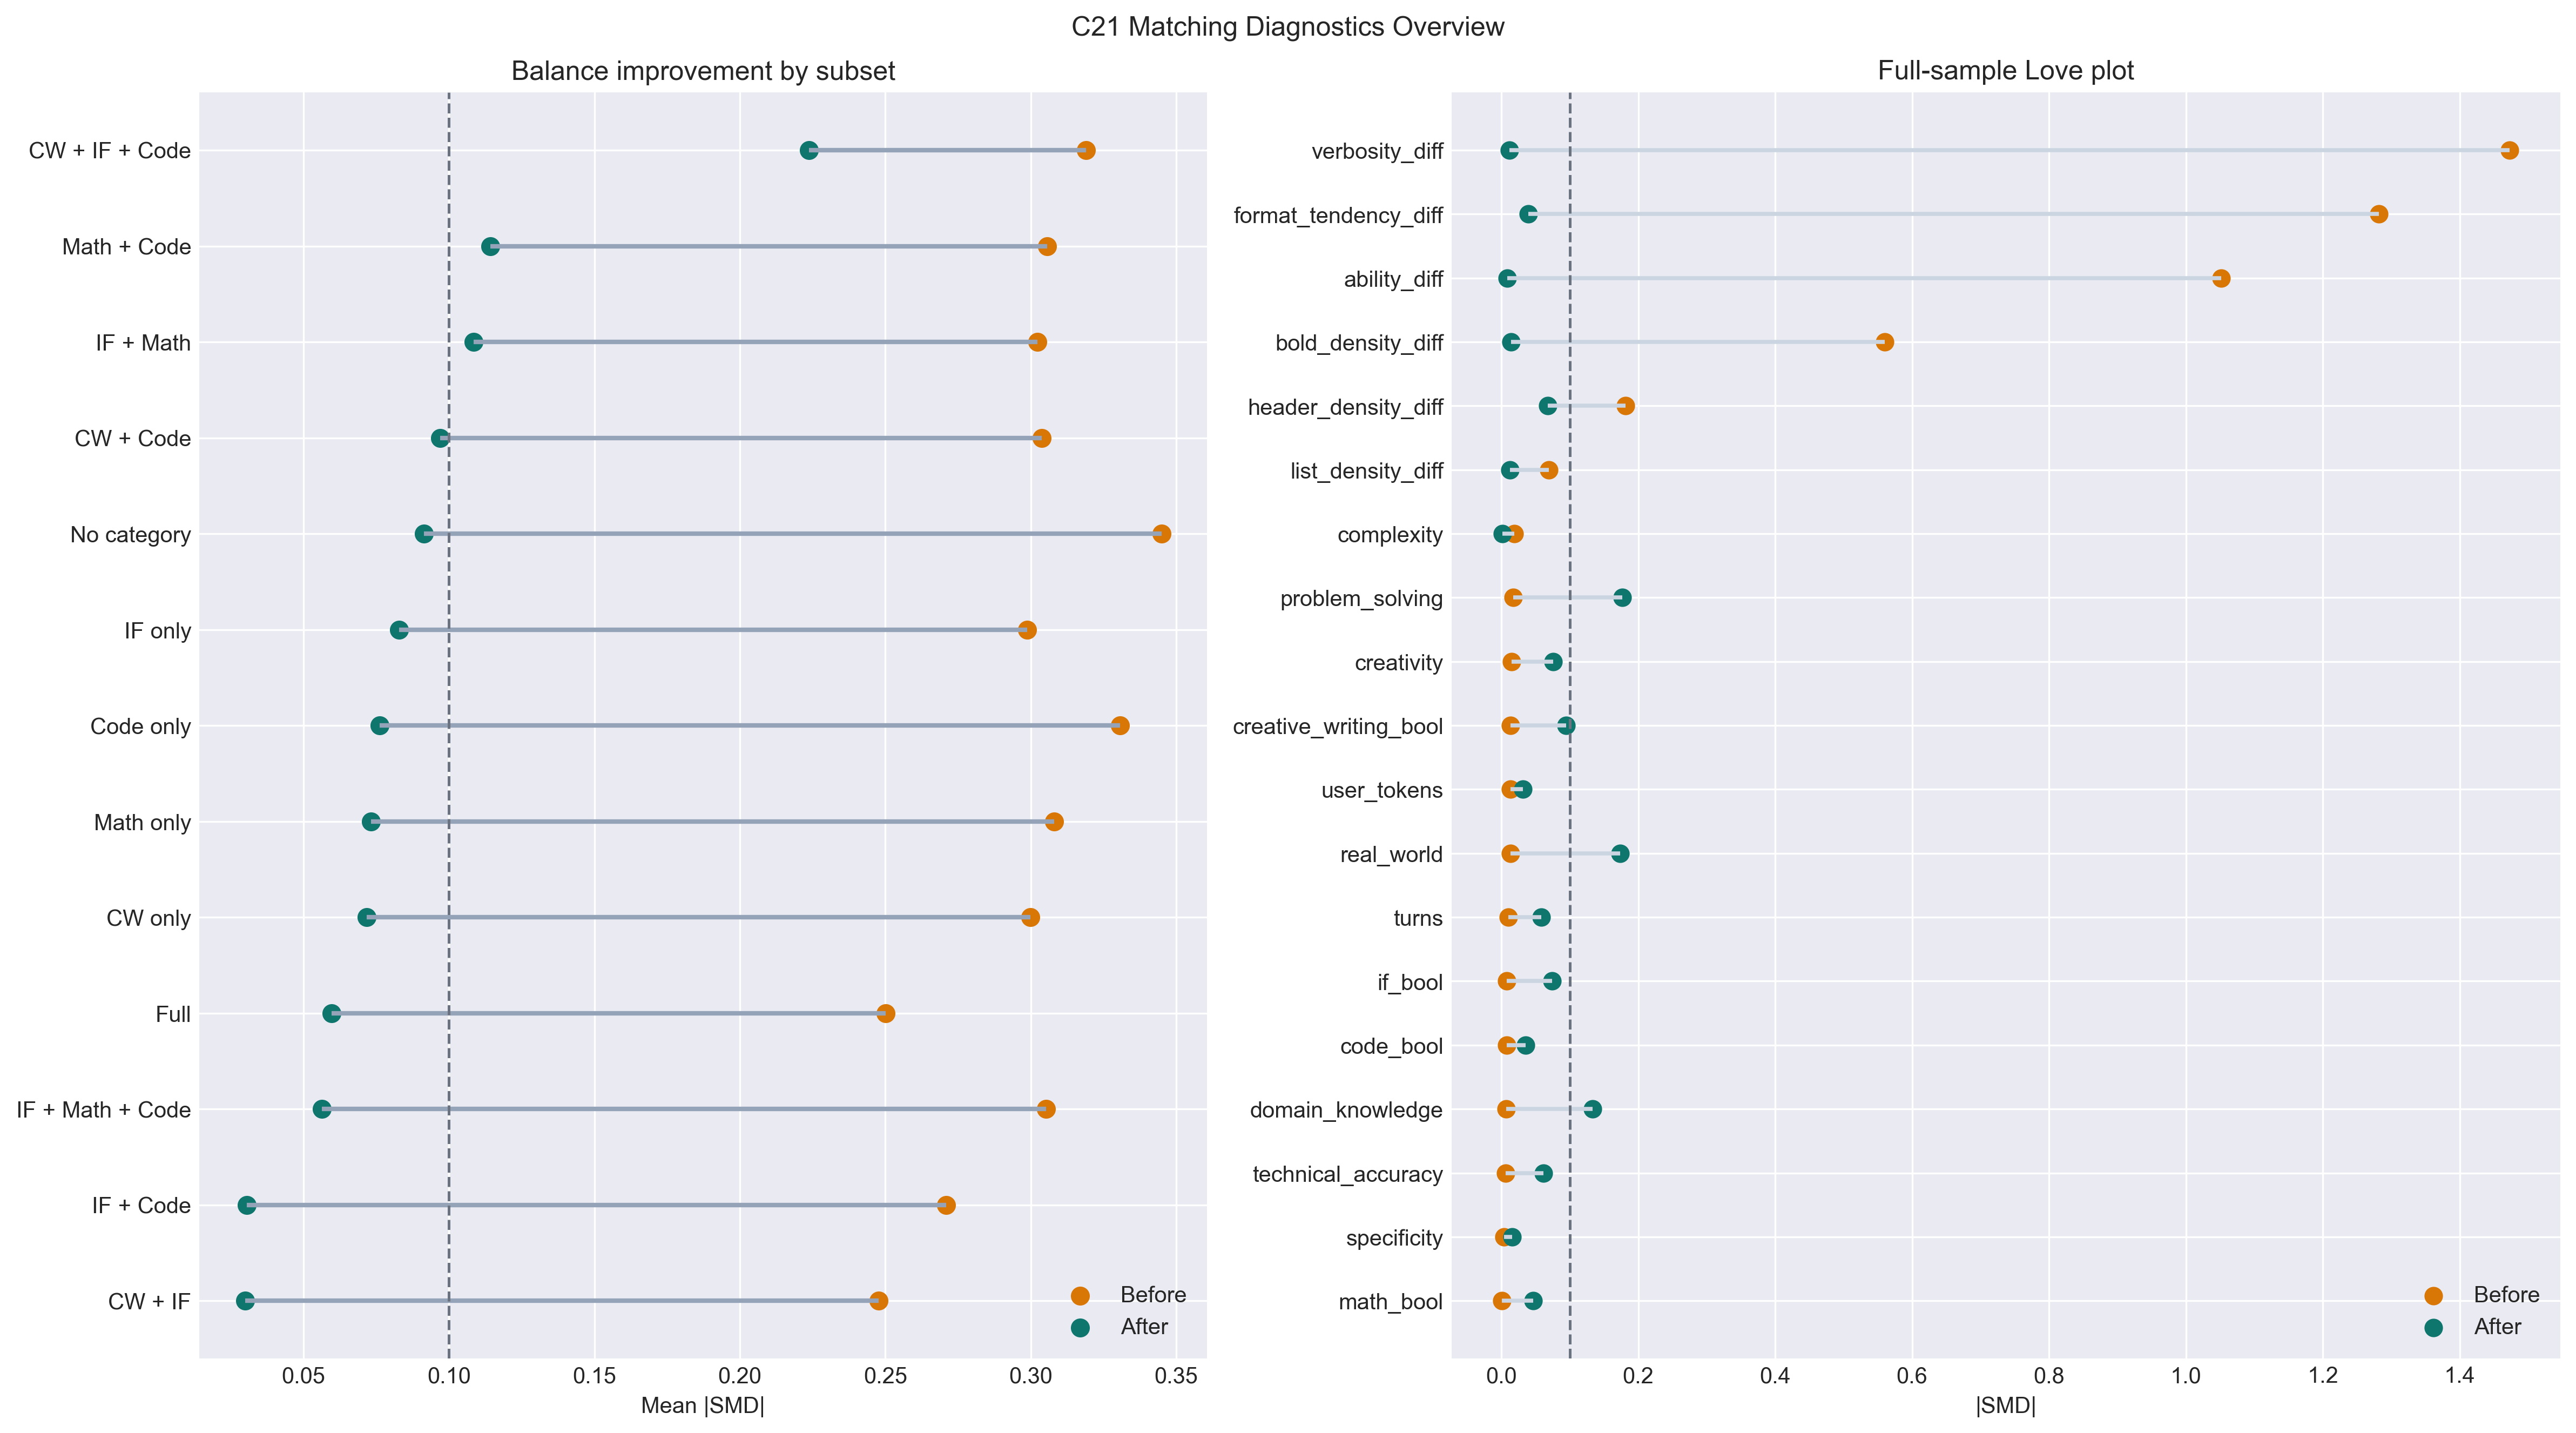
\includegraphics[width=0.9\textwidth]{figures/P12_matching_diagnostics_overview.png}
\caption{匹配诊断总览图}
\label{fig:matching}
\end{figure}

% ==================== 第七章 ====================
\section{机制探索与路径分析}

\subsection{路径分析框架与变量设定}
前述分析已经证明，长度偏好和部分格式偏好在控制混淆后仍然存在，但这仍主要停留在“是否存在”与“是否稳健”的层面。为了进一步考察这些变量如何共同进入最终偏好判断，本文构建了结构方程模型，并将 \tokendiff、\headerD 和 \boldD 作为主模型路径层变量；扩展模型额外加入 \listD，仅作敏感性分析。

模型的外生层变量包括任务类型、质量维度、模型能力差、冗长度风格差、格式倾向差、用户输入长度与回合数等控制项，结果层变量为 \winner。这样的设计使本文能够同时观察能力差异、风格差异与路径层变量对偏好结果的影响。

从方法类型上看，本文使用的是观测变量 SEM，而不是潜变量测量模型。也就是说，模型并不试图把“质量”“结构化程度”抽象为潜在因子，而是直接使用已经在前序分析中定义好的可观测变量建模。这种处理更贴合本项目的数据条件，也能保证 SEM 与前文的逻辑回归、IPW、PSM 使用的是同一套分析口径，而不是重新发明一套难以对照的新变量体系。

\subsection{模型拟合与结构关系检验}
主模型使用 78,970 条样本进行估计，拟合指标表现良好，CFI=0.9998，TLI=0.9998，RMSEA=0.0030。扩展模型虽然在数值上给出更高的拟合指标，但由于 \listD 在前序分析中被识别为敏感性变量，本文仍以主模型作为正式结论依据。

从关键路径估计看，\winner 对 \tokendiff、\headerD 和 \boldD 的路径系数均为正，表明在控制外生变量后，长度差、标题密度差和粗体密度差都与偏好方向正相关。同时，\ability、\verbosity 和 \formatt 会显著影响路径层变量，说明偏好中的形式特征确实嵌入在更复杂的模型风格结构中。

这里对拟合指标的解读需要保持克制。CFI 和 TLI 接近 1、RMSEA 接近 0，说明主模型作为一张整体路径网络，能够较好贴合样本中的协方差结构；但这并不意味着模型设定就是唯一正确的。主模型之所以仍优先于扩展模型，不是因为扩展模型拟合“更差”，而是因为列表变量在前序稳健性分析中并未表现出足够稳定的独立效应。换言之，本文选择主模型，是基于“拟合充分 \(+\) 理论简洁 \(+\) 与前序证据一致”的综合原则，而不是单纯挑选一个拟合值最好看的模型。

\subsection{长度与格式特征的作用路径分析}
为了避免把 SEM 结果压缩成一句“路径显著”，本节按变量链条逐条解释主模型中的关键路径。首先看 \tokendiff 到 \winner 的路径系数，其值为 0.6073，方向为正，说明在控制能力差、风格差、任务类型和质量维度后，A 侧相对更长时，A 侧获胜概率仍倾向上升。这条路径对应的是“长度差作为路径层变量对偏好的直接贡献”，也是前文长度稳健性结果在路径框架中的延续。

其次，\headerD 到 \winner 的路径系数为 0.0173，\boldD 到 \winner 的路径系数为 0.0215，二者方向同样为正。虽然这两个数值明显小于长度路径系数，但它们在 Bootstrap 区间中都排除了 0，说明标题和粗体并不只是“附带好看”的装饰，而是在控制长度和模型风格后，仍然能独立提高被选择概率。换言之，用户对结构化表达的奖励，并不完全依赖文本更长这一前提。

第三，\ability 到 \winner 的直接路径系数为 0.1549，表明模型能力差越偏向 A，A 侧越容易直接获胜。这一路径代表的是“能力优势本身”对偏好的贡献，而不是通过长度或格式转译后的贡献。与之对应，\ability 到 \tokendiff 的路径系数为 \(-0.0218\)，且“能力 \(\rightarrow\) 长度 \(\rightarrow\) 偏好”的 Bootstrap 区间跨 0，这也说明能力更强的模型并不是稳定地靠“写得更长”来赢。对照来看，“能力 \(\rightarrow\) 标题密度 \(\rightarrow\) 偏好”和“能力 \(\rightarrow\) 粗体密度 \(\rightarrow\) 偏好”的间接效应区间均排除 0，提示更强模型更可能通过更有效的结构组织，而不是单纯拉长文本，来获得额外偏好优势。

第四，\verbosity 到 \tokendiff 的路径系数为 0.5020，而 \verbosity 到 \winner 的直接路径系数为 \(-0.2608\)。两条路径合起来说明：冗长度风格确实会推高长度差，但这种“更会写长”并不等于“更受喜欢”；在控制住实际长度差和格式差之后，纯粹的冗长倾向反而与偏好呈负向关系。这一结果有助于区分“有效长度”与“无效冗长”：前者可能带来信息充分感，后者则可能表现为啰嗦和低效率。

第五，\formatt 到 \winner 的直接路径系数为 \(-0.0236\)，且其 Bootstrap 区间跨 0；但 \formatt 到 \headerD 的路径系数为 0.6551，到 \boldD 的路径系数为 0.8300，且通过标题与粗体进入 \winner 的间接路径区间均排除 0。这也说明“模型整体更偏好格式化表达”本身并不会自动转化为更高偏好，真正被用户奖励的是可以被直接感知的具体格式策略，如清晰的小标题和重点强调，而不是抽象的格式倾向标签。

第六，主模型中允许 \headerD 与 \boldD 存在协方差。这一设定的含义并不是“标题导致粗体”或“粗体导致标题”，而是承认二者作为结构化表达策略常常共同出现。它提醒我们：在机制解释中，不应把所有共现都误读为因果顺序。有些关系只是表示两种风格在未观测层面仍共享同一组织倾向。

\subsection{直接效应、间接效应与结构分解}
Bootstrap \(95\%\) 置信区间的解释需要结合重采样规模一起阅读。本文主模型的 bootstrap 设定为 50 次，最终有效重采样为 46 次，未成功的 4 次来自重采样样本在 semopy 拟合阶段失败。这样一来，相关区间更适合作为机制层的辅助证据，而不宜被当作高精度估计。就有效重采样结果而言，标题密度直接效应的区间为 \([0.0086,0.0263]\)，粗体密度直接效应的区间为 \([0.0096,0.0361]\)，均排除 0；而长度直接效应的区间为 \([-0.0690,1.5056]\)，跨越 0。这并不否定长度优势在前述检验中的稳健存在，而是提示长度变量在机制层面可能同时承载长度、模型能力和回答组织方式等多重代理含义，因而其路径解释比标题和粗体更复杂。

与此同时，格式倾向的直接效应区间跨 0，但“格式倾向 \(\rightarrow\) 标题密度 \(\rightarrow\) 偏好”和“格式倾向 \(\rightarrow\) 粗体密度 \(\rightarrow\) 偏好”的间接效应区间均排除 0。这也说明某些模型风格并不是直接让回答更容易获胜，而是通过生成更具结构性的标题与重点标记，间接提高被选择概率。

这样一来，H4 可以得到谨慎支持：长度和关键格式变量确实共同进入了偏好形成过程，但标题与粗体的路径更接近可直接解释的形式效应，而长度更像一个在统计层面稳健、在机制层面仍需进一步拆分的综合性代理变量。

若从效应分解的角度来读，上述结果实际上对应三种不同的变量角色。长度差既是前文最稳健的统计关联变量，又在路径层面呈现“点估计为正但区间跨 0”的情形，因而更像一个混合性路径变量，兼有效信息承载与模型风格代理两种属性。标题密度与粗体密度则更接近“局部可解释路径变量”，即它们虽然效应规模不大，但方向稳定、区间清晰，且与前文稳健性分析结论高度一致。能力差与格式倾向差则更像“上游驱动变量”，它们的重要性不只体现在直接路径，更体现在它们如何把影响传导给长度与格式路径层。

从论文写作角度看，这一分解方式也意味着本文不能把“长度、标题、粗体都显著”写成同质化结论。更精确的写法应是：标题与粗体具备更清晰的直接路径支持；长度则在现象层和稳健性层都成立，但在机制层面仍需与冗长风格、模型能力和任务适配性进一步拆分。

\subsection{路径分析的解释边界与适用范围}
尽管 SEM 为本文提供了比单一回归更丰富的解释框架，但其路径解释仍然有边界。首先，模型设定上，本文使用的是观测变量路径模型，而不是基于实验设计的强因果识别框架，因而这里的“直接效应”和“间接效应”更适合解释为理论一致、统计上可支持的传导结构，而不应被写成严格因果定论。其次，路径方向本身依赖研究者的理论设定，如把能力差和风格差放在外生层、把长度差和格式密度差放在路径层，是基于前序分析和研究问题做出的建模选择，而不是数据本身自动生成的真理结构。

第三，Bootstrap 区间能够缓解间接效应乘积分布不对称的问题，但不能替代对遗漏变量的控制。与此同时，本文 SEM 的 bootstrap 设定为 50 次、有效重采样为 46 次，因而区间估计更适合作为方向性与稳健性辅助信息，而非高精度参数估计。如果未来引入更细粒度的回复质量指标、信息覆盖率指标或局部冗余指标，并提高重采样次数，长度路径的解释有望进一步细化。也正因为如此，本研究把 SEM 的主要贡献界定为“把偏好存在性研究推进到机制分解层面”，而不是宣称已经完整识别出偏好形成的全部因果链条。

\begin{figure}[htbp]
\centering
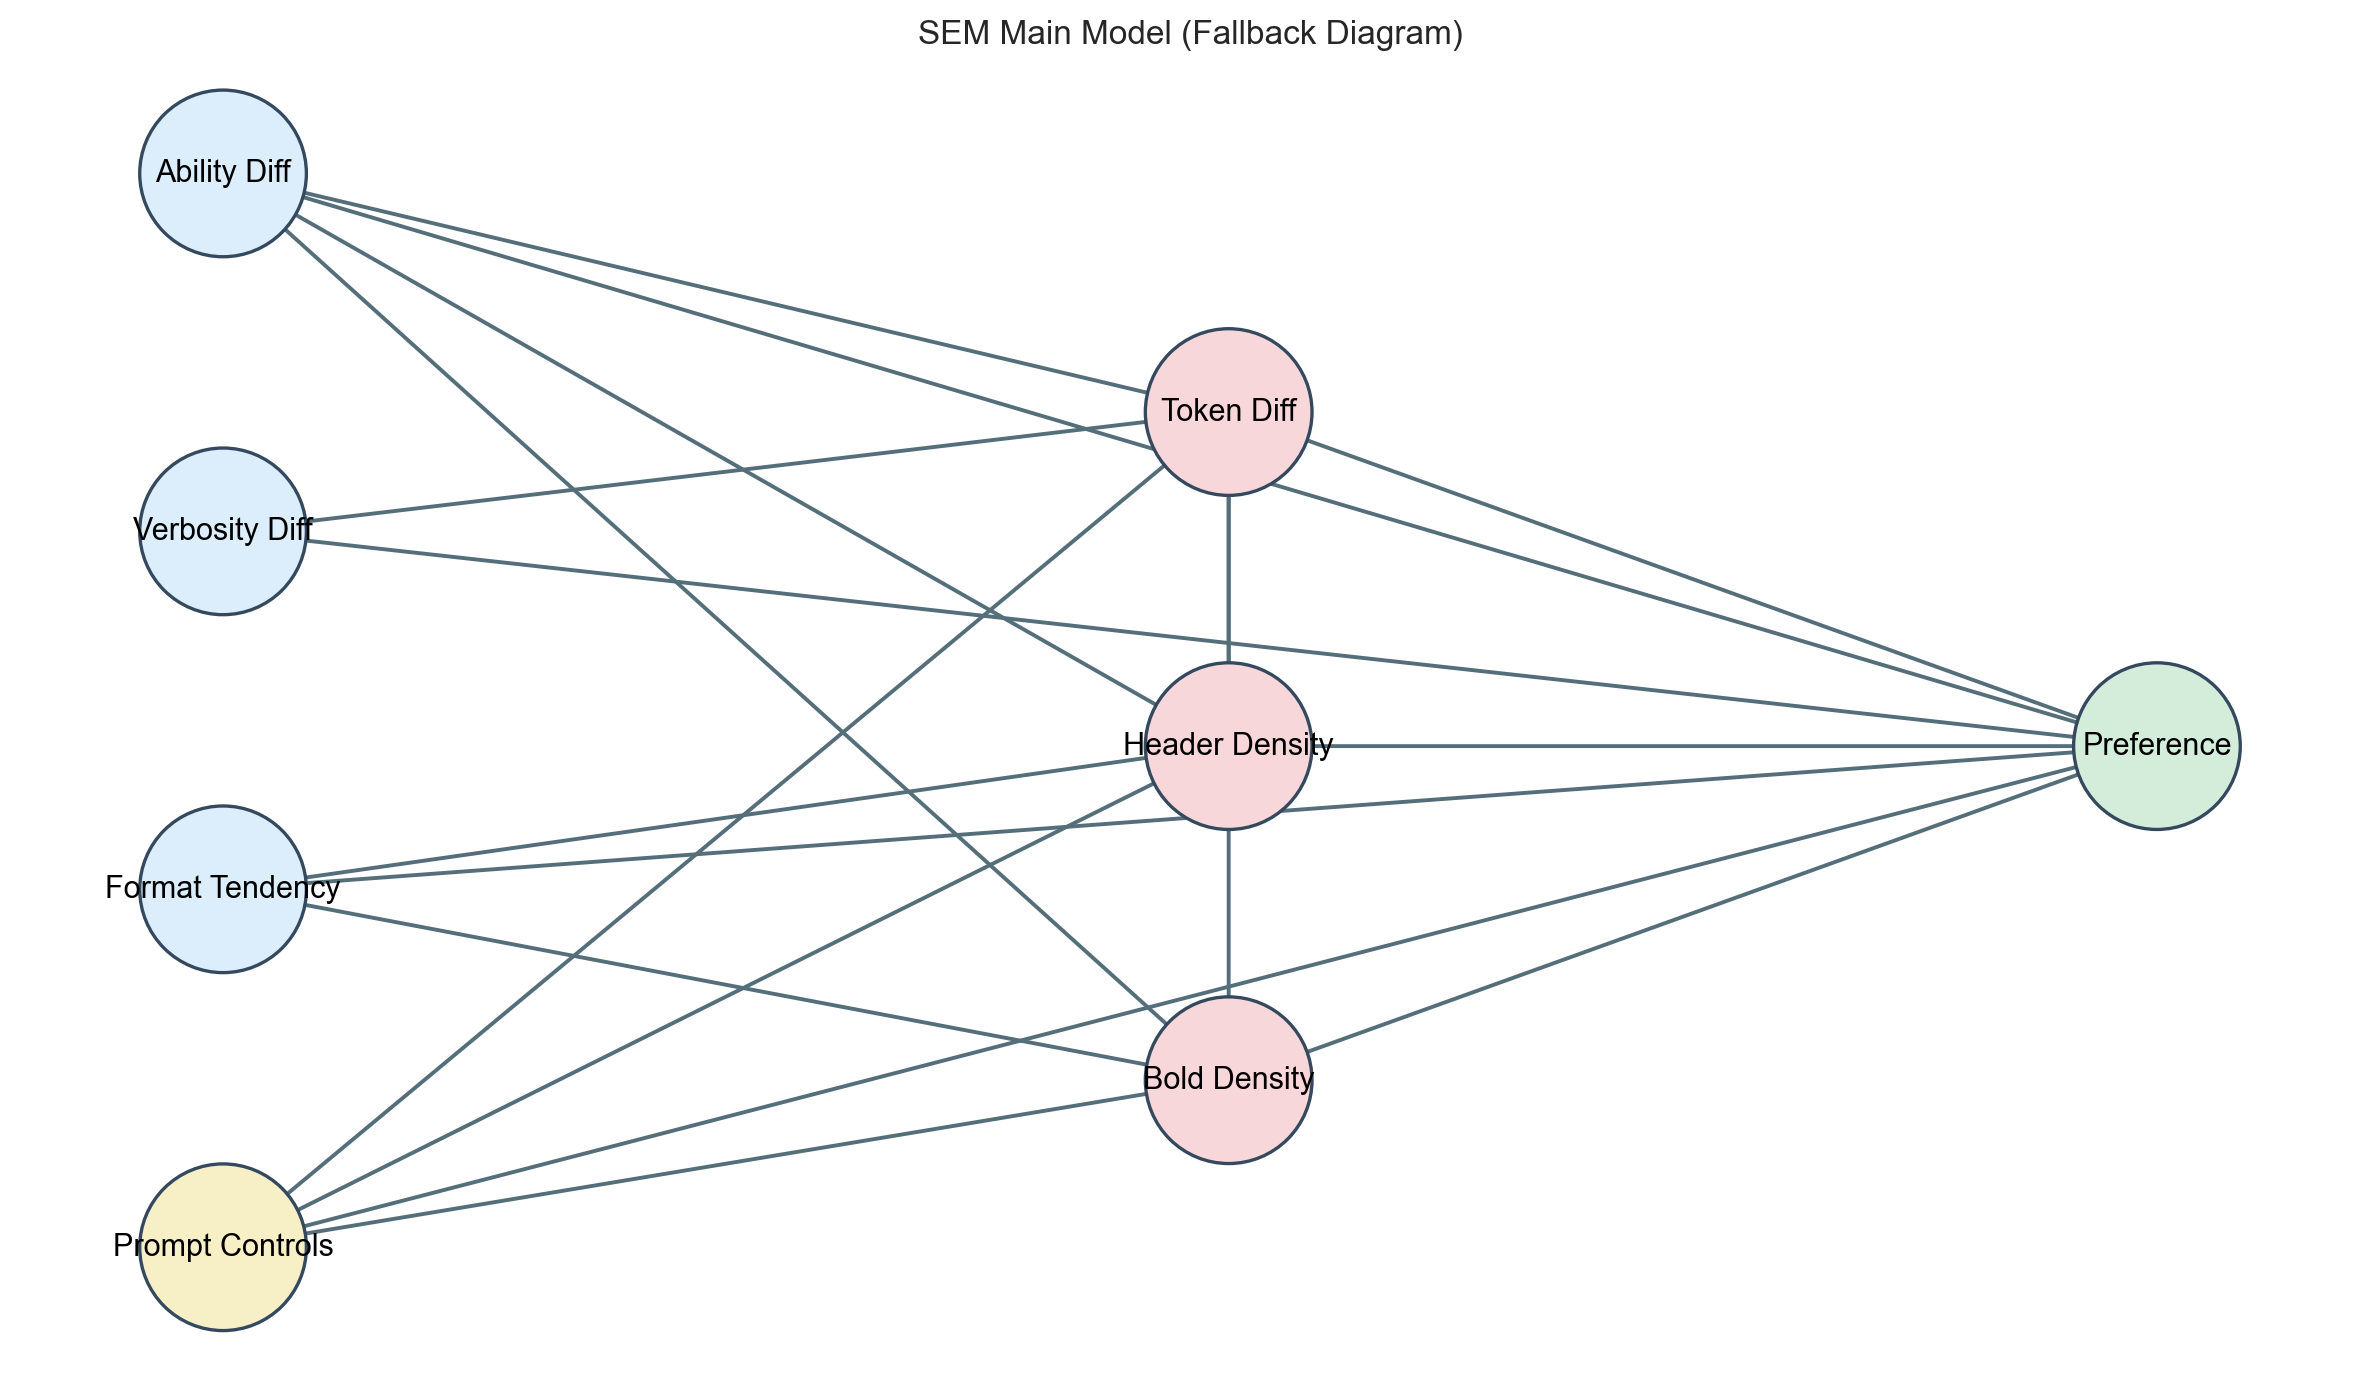
\includegraphics[width=0.9\textwidth]{figures/P13_sem_path_diagram.png}
\caption{SEM 路径图}
\label{fig:sem_path}
\end{figure}

\begin{table}[htbp]
\centering
\caption{SEM 效应分解与 Bootstrap 区间}
\label{tab:sem_effects}
\begin{tabular}{lrrrrl}
\toprule
效应 & 点估计 & Bootstrap 均值 & Bootstrap 标准差 & 95\%置信区间 & 95\% CI 排除 0 \\
\midrule
长度直接效应 & 0.607 & 0.298 & 0.474 & \([-0.069,1.506]\) & 否 \\
标题密度直接效应 & 0.017 & 0.017 & 0.006 & \([0.009,0.026]\) & 是 \\
粗体密度直接效应 & 0.021 & 0.022 & 0.007 & \([0.010,0.036]\) & 是 \\
能力直接效应 & 0.155 & 0.149 & 0.020 & \([0.122,0.191]\) & 是 \\
能力 \(\rightarrow\) 长度 \(\rightarrow\) 偏好 & \(-0.013\) & \(-0.005\) & 0.015 & \([-0.050,0.011]\) & 否 \\
能力 \(\rightarrow\) 标题密度 \(\rightarrow\) 偏好 & 0.006 & 0.006 & 0.003 & \([0.003,0.012]\) & 是 \\
能力 \(\rightarrow\) 粗体密度 \(\rightarrow\) 偏好 & 0.003 & 0.003 & 0.001 & \([0.002,0.006]\) & 是 \\
能力总间接效应 & \(-0.004\) & 0.004 & 0.016 & \([-0.041,0.027]\) & 否 \\
能力总效应 & 0.151 & 0.153 & 0.011 & \([0.139,0.169]\) & 是 \\
词汇性 \(\rightarrow\) 长度 \(\rightarrow\) 偏好 & 0.305 & 0.147 & 0.241 & \([-0.035,0.784]\) & 否 \\
格式倾向直接效应 & \(-0.024\) & \(-0.033\) & 0.028 & \([-0.079,0.008]\) & 否 \\
格式倾向 \(\rightarrow\) 标题密度 \(\rightarrow\) 偏好 & 0.011 & 0.011 & 0.004 & \([0.005,0.018]\) & 是 \\
格式倾向 \(\rightarrow\) 粗体密度 \(\rightarrow\) 偏好 & 0.018 & 0.018 & 0.006 & \([0.008,0.030]\) & 是 \\
格式倾向总间接效应 & 0.029 & 0.030 & 0.009 & \([0.019,0.046]\) & 是 \\
\bottomrule
\end{tabular}
\end{table}

% ==================== 第八章 ====================
\section{总结与讨论}

本文最具理论意义的发现，并不只是再次确认长度偏好存在，而是把表层形式偏差拆分为不同层次的统计对象。长度粗效应中有 \(60.74\%\) 可由任务类型、质量维度以及模型能力与风格差异解释，说明如果只看原始相关，长度优势会被明显放大；格式偏差内部则呈现显著异质性，标题与粗体在净效应和处理效应框架下都保持独立正向作用，列表则主要表现为长度扩张和文本组织方式的伴生信号；长度虽然在现象层最为稳健，却在 SEM 直接路径上区间跨 0，因而更适合被理解为复合代理变量，而非单一路径因素。这一结果与 Li 等人对人类偏好属性的拆解研究形成呼应，但本文还进一步量化了长度粗效应中的混淆份额，并将格式变量内部的异质性纳入同一框架；它也与 Zhang 等人关于格式偏差可以被对齐过程放大的发现相衔接，但本研究指出真正需要优先防范的并不是“所有格式”，而是标题与粗体这类更稳定的结构线索。

从偏好对齐理论看，Shen 等人指出奖励模型会把“更长 \(=\) 更好”学习为捷径，而本文从数据源头补足了这一机制链条：人类偏好数据本身就包含系统性长度优势与部分格式优势，因而奖励模型并不是凭空产生偏差，而是在既有偏好结构上继续放大。就此而言，偏好数据不是中性的训练资源，而是同时混合内容质量判断与表层启发式判断的复合信号。这一发现也扩展了 reward hacking 相关讨论。如果对齐研究仍沿用“收集偏好数据—训练奖励模型—事后发现捷径”的被动路径，那么很多表层偏差会在训练前端就被写入目标函数；更合理的范式应是把数据审计前置，把研究重心从“如何优化对齐算法”延伸到“对齐目标本身是否可靠”。

在实践层面，本文结果对应四项可操作的去偏策略。在偏好数据构建阶段，应优先实施轮次审计、长度匹配和格式平衡，对于多轮会话数据，研究者应先确认研究单位是否仍对应当前比较单元，对于长度差异过大的样本，可在采样或分析阶段单独标记，以降低“长即优”的先验优势。在奖励模型训练阶段，应把长度与格式变量视为需要显式监控的捷径特征，而非默认可直接吸收的输入信号，PoE、响应条件化建模和后验校准等方法，都可以理解为将主奖励信号与表层代理信号分离的实现路径。在自动评价器和基准测试设计阶段，应报告长度控制后的排名，或至少同步报告原始排名与校正排名，避免把对未经审计偏好数据的拟合误当作评价能力提升。在经验研究规范层面，后续偏好研究应同时报告粗相关、控制混淆后的净效应以及至少一种处理效应估计，而不宜仅凭单一显著性结果给出强结论。

本文仍存在四方面局限。第一，研究对象主要来自 LMArena 单一偏好数据源，虽然规模较大且有真实交互痕迹，但与专业标注场景之间仍存在任务分布与标注制度差异，因此推广到其他平台时应保持谨慎。第二，本研究对模型能力与风格的代理变量采用全量样本一次性估计后映射到配对层，未使用留一法或交叉验证，因而这些代理量更适合作为控制项，而非外部可推广评分。第三，本文聚焦长度、标题、列表和粗体等可操作化较强的形式特征，尚未将礼貌性、语气风格、局部冗余模式和信息覆盖度等更细粒度因素纳入统一框架。第四，SEM 仍基于观测数据，且本研究的 bootstrap 设定为 50 次、有效重采样为 46 次，4 次失败来自重采样样本拟合未收敛，因此第七章的区间估计更适合作为机制层的辅助证据，而不应被理解为高精度因果识别结果。

综合来看，本文基于 LMArena 人类偏好数据，围绕长度偏差与格式偏差形成了四点主要结论。其一，经过数据审计与清洗后，本文确认首轮评价记录构成了更一致的研究对象，只保留 evaluation\_order 等于 1 的处理，实质上是对长度测量口径的统一，而不是经验性删样。其二，长度偏好在描述统计、正式检验、调整逻辑回归、IPW 和匹配诊断中都表现出稳定优势，全量样本中胜者更长比例为 \(62.21\%\)，中位长度差为 \(+125\) tokens，在控制混淆后，长度净效应与处理效应仍保持显著；但 SEM 结果显示长度直接效应区间跨 0，因而其稳健性主要体现在现象层与控制混淆后的稳健性层，而不宜被简化为单一路径效应。其三，格式偏好内部存在明显分化，标题和粗体在密度分析与稳健性框架下仍能保留独立正向效应，而列表在本文采用的密度指标与控制框架下更接近长度扩张的伴生信号，不宜作为主结论单独强调。其四，路径分析显示，人类偏好数据中的形式偏差并不是完全停留在表层相关，标题密度与粗体密度的直接路径有较清晰的统计支持，而长度虽然与偏好稳健相关，但在机制层面仍承载代理含义，说明偏好形成并不是单一路径驱动。

在理论层面，本文将 RLHF 偏好数据中的长度偏差与格式偏差置于统一框架之下，不再把它们视作彼此孤立的评测现象。与 Li 等人对偏好属性权重的拆解相比，本研究还进一步量化了长度粗效应的混淆份额；与 Shen 等人对奖励模型长度捷径的讨论相比，这项研究补充了捷径源头来自数据层的经验证据；与 Zhang 等人关于格式偏差放大的研究相比，文中还进一步识别出标题、粗体与列表之间的稳定性分化。在方法层面，本文建立了一条从数据审计、存在性识别、净效应估计到多框架稳健性验证和 SEM 机制探索的连续分析链，这一框架不仅适用于本研究，也可以为后续关于位置偏差、语气偏差和谄媚性偏差等问题的研究提供可复用范式；实践上，evaluation\_order 污染识别、格式密度指标构造以及 OR、ATE、SMD 与路径系数的联合使用，共同构成了这项研究可迁移的方法学贡献。未来研究可以从四个方向继续推进：一是扩展到更多平台、语言和评价协议，检验本文结论的外部有效性；二是构造更丰富的回复级路径层变量，如结构完整度、证据覆盖率和局部信息冗余度，以进一步拆解长度效应；三是对 no\_category 子集做更细粒度再分类，识别任务语境与形式偏好之间的交互关系；四是基于本研究识别出的偏差模式，尝试构造去偏后的偏好训练数据，并检验其是否能够改善对齐训练质量。

\begin{thebibliography}{99}

\bibitem{li2025multi} 黎宇声. 多目标对齐大语言模型的强化学习策略研究[D]. 电子科技大学, 2025.

\bibitem{hu2024explaining} Hu Zhengyu, et al. Explaining Length Bias in LLM-Based Preference Evaluations[EB/OL]. arXiv, 2024.

\bibitem{liu2025format} Liu Jiacheng, et al. Format as a Prior: Quantifying and Analyzing Bias in LLMs for Heterogeneous Data[EB/OL]. arXiv, 2025.

\bibitem{li2024dissecting} Li Junlong, et al. Dissecting Human and LLM Preferences[EB/OL]. arXiv:2402.11296, 2024.

\bibitem{shen2023loose} Shen Wei, et al. Loose Lips Sink Ships: Mitigating Length Bias in Reinforcement Learning from Human Feedback[EB/OL]. arXiv, 2023.

\bibitem{dubois2024length} Dubois Yann, et al. Length-Controlled AlpacaEval: A Simple Way to Debias Automatic Evaluators[EB/OL]. arXiv:2404.04475, COLM 2024.

\bibitem{zhang2024lists} Zhang Xuancheng, et al. From Lists to Emojis: How Format Bias Affects Model Alignment[EB/OL]. arXiv, 2024.

\bibitem{park2024offsetbias} Park Junsoo, et al. OffsetBias: Leveraging Debiased Data for Tuning Evaluators[EB/OL]. arXiv:2407.06551, EMNLP Findings 2024.

\bibitem{han2023causal} 韩明月. 因果推断视角下自然语言处理任务中的虚假相关性研究[D]. 上海财经大学, 2023.

\bibitem{ouyang2022training} Ouyang Long, et al. Training Language Models to Follow Instructions with Human Feedback[C]//Advances in Neural Information Processing Systems (NeurIPS). 2022. arXiv:2203.02155.

\bibitem{rafailov2023direct} Rafailov Rafael, et al. Direct Preference Optimization: Your Language Model Is Secretly a Reward Model[C]//NeurIPS. 2023. arXiv:2305.18290.

\bibitem{huang2025posthoc} Huang Zeyu, et al. Post-hoc Reward Calibration: A Case Study on Length Bias[C]//The Thirteenth International Conference on Learning Representations (ICLR). 2025.

\bibitem{do2024llms} Do Xuan Long, et al. LLMs Are Biased Towards Output Formats! Systematically Evaluating and Mitigating Output Format Bias of LLMs[EB/OL]. arXiv, 2024.

\bibitem{sun2023principle} Sun Zhiqing, et al. Principle-Driven Self-Alignment of Language Models from Scratch with Minimal Human Supervision[C]//NeurIPS. 2023.

\bibitem{li2024ruler} Li Jiaming, et al. Ruler: A Model-Agnostic Method to Control Generated Length for Large Language Models[EB/OL]. arXiv:2409.18943, 2024.

\bibitem{gan2026biaxis} Gan Jialing, et al. BiAxisAudit: A Novel Framework to Evaluate LLM Bias Across Prompt Sensitivity and Response-Layer Divergence[EB/OL]. arXiv:2605.09041, 2026.

\bibitem{sharma2024towards} Sharma Mrinank, et al. Towards Understanding Sycophancy in Language Models[C]//Proceedings of ACL. 2024. arXiv:2310.13548.

\bibitem{koo2024benchmarking} Koo Ryan, et al. Benchmarking Cognitive Biases in Large Language Models as Evaluators[C]//Proceedings of ACL. 2024. arXiv:2309.17012.

\bibitem{wang2025beyond} Wang Chaoqi, et al. Beyond Reward Hacking: Causal Rewards for Large Language Model Alignment[EB/OL]. arXiv:2501.09620, 2025.

\bibitem{wang2026reward} Wang Xiaohua, et al. Reward Hacking in the Era of Large Models: Mechanisms, Emergent Misalignment, Challenges[EB/OL]. arXiv:2604.13602, 2026.

\bibitem{kim2025mitigating} Kim Hyeonji, Oh Sujeong, Lee Sanghack. Mitigating Length Bias in RLHF through a Causal Lens[EB/OL]. arXiv:2511.12573, 2025.

\bibitem{cai2025disentangling} Cai Jianfeng, et al. Disentangling Length Bias in Preference Learning via Response-Conditioned Modeling[EB/OL]. arXiv:2502.00814, 2025.

\bibitem{ye2025rectifying} Ye Wenqian, Zheng Guangtao, Zhang Aidong. Rectifying Shortcut Behaviors in Preference-based Reward Learning[EB/OL]. arXiv:2510.19050, 2025.

\end{thebibliography}

\end{document}